\documentclass[11pt]{article}

\usepackage[margin=22mm]{geometry}
\usepackage{amsmath}
\usepackage{array}
\usepackage{booktabs}
\usepackage{graphicx}
\usepackage{tikz}
\usepackage{url}
\usetikzlibrary{arrows.meta,calc,positioning}

\title{Single-Bend Analytic Placement Tests}
\author{OPALX element placing sandbox}
\date{\today}

\newcommand{\degree}{^\circ}
\newcommand{\code}[1]{\texttt{#1}}
\newcommand{\vect}[1]{\boldsymbol{#1}}

\tikzset{
  axis/.style={-{Latex[length=2mm]}, thin, black!70},
  design/.style={very thick, blue!70!black},
  fringe/.style={thick, dashed, orange!80!black},
  pose/.style={-{Latex[length=2mm]}, thick, green!45!black},
  poleface/.style={thick, green!45!black},
  poleangle/.style={-{Latex[length=1.4mm]}, thick, green!45!black},
  monitor/.style={thick, red!70!black},
  marker/.style={circle, fill=black, inner sep=1.4pt},
  note/.style={font=\scriptsize, align=left, fill=white, inner sep=1.5pt}
}

\begin{document}
\maketitle

\section{Purpose}

The sandbox inputs
\begin{center}
\begin{tabular}{@{}ll@{}}
\code{SBEND} placement & \code{sandbox/test-sbend-1/test-sbend-1.in} \\
\code{SBEND} vertical focusing & \code{sandbox/test-sbend-2/test-sbend-2.in} \\
\code{RBEND} placement & \code{sandbox/test-rbend-1/test-rbend-1.in} \\
\code{RBEND} vertical focusing & \code{sandbox/test-rbend-2/test-rbend-2.in}
\end{tabular}
\end{center}
exercise the OPALX-native analytic \code{SBEND} and \code{RBEND} without field
maps, using the native analytic bend model and explicit poses.  The first test
of each bend type is a placement consistency test.  The second test adds a
vertical offset and checks the pole-face/fringe-field focusing against old
OPAL 2022.1.

Both tests use explicit element posing:
\[
  (X,Y,Z,\Theta,\Phi,\Psi),
\]
where \((X,Y,Z)\) is the placed body-frame origin and \(\Theta\) is the body
rotation about the global \(Y\)-axis in the \(X\)-\(Z\) drawing plane.  The
figures use this global \(X\)-\(Z\) projection; for these horizontal-bend tests
the body pose has \(Y=0\), normal to the drawing plane.

\section{Bend Models}

The two analytic bend elements describe the same physical dipole problem from
different geometric conventions.  Both are intended to give the design bend
angle \(\theta\) from the integrated dipole field.  The distinction is the
reference frame used to define the magnet body, the meaning of the length
attribute, and therefore the pole-face angles at which the circular reference
orbit enters and leaves the magnet.

\subsection{Physical distinction}

\code{SBEND} is a sector bend.  The reference orbit is a circular arc and the
natural hard-edge pole faces are radial.  With no additional pole-face angles
the beam enters and exits normal to the pole faces, so no thin-edge focusing is
introduced by the geometry itself.

\code{RBEND} is a rectangular bend.  The magnet body is straight, while the
reference orbit is still a circular arc through the dipole field.  The orbit
therefore crosses the entrance and exit pole faces at nonzero edge angles.  For
the same \(\theta\), this makes edge and fringe focusing part of the natural
rectangular-bend model.

\subsection{OPALX \code{SBEND} model}

For the sandbox \code{SBEND} tests
\[
  L_\mathrm{chord} = 1.0\ \mathrm{m},\qquad
  \theta = 45\degree = \frac{\pi}{4},\qquad
  R = \frac{L_\mathrm{chord}}{2\sin(\theta/2)}
    = 1.3065629649\ \mathrm{m}.
\]
For parser-created \code{SBEND}, OPALX follows old OPAL and treats \code{L} as
the chord.  The placed sector arc length and curvature are therefore
\[
  L_\mathrm{ref} = R\theta
  = L_\mathrm{chord}\frac{\theta}{2\sin(\theta/2)}
  = 1.0261721530\ \mathrm{m},
  \qquad
  h = \frac{\theta}{L_\mathrm{ref}} = \frac{1}{R}
    = 0.7653668647\ \mathrm{m}^{-1}.
\]
OPALX stores this as a \code{PlanarArcGeometry}.  The body-frame origin is at
the arc midpoint, so the body coordinate \(s\) runs from
\(-L_\mathrm{ref}/2\) to \(+L_\mathrm{ref}/2\).  The local sector orbit is the
standard sector-bend reference-orbit convention used in first-order beam
dynamics \cite{holzer2018,bmad}:
\[
  \vect r(s) =
  \begin{pmatrix}
    \dfrac{\cos(hs)-1}{h}\\[1.0ex]
    0\\[0.5ex]
    \dfrac{\sin(hs)}{h}
  \end{pmatrix},
  \qquad
  \vect t(s) =
  \begin{pmatrix}
    -\sin(hs)\\
    0\\
    \cos(hs)
  \end{pmatrix}.
\]
For \(L_\mathrm{chord}=1\ \mathrm{m}\) and \(\theta=45\degree\),
\[
  \vect r_\mathrm{entry}
  = (-0.0994561837,\,0,\,-0.5000000000)\ \mathrm{m},
  \qquad
  \vect r_\mathrm{exit}
  = (-0.0994561837,\,0,\,0.5000000000)\ \mathrm{m}.
\]

\subsection{OPALX \code{RBEND} model}

The \code{RBEND} tests use the same bend angle and field model as the
\code{SBEND} tests, but the body geometry is rectangular.  The input length is
the straight body length,
\[
  L_\mathrm{rect}=1.0\ \mathrm{m},\qquad
  \theta=45\degree,\qquad
  E_1=0,\qquad E_2=\theta .
\]
Old OPAL uses the pole-face chord radius for a rectangular bend,
\[
  R_\mathrm{CH} =
    \frac{L_\mathrm{rect}}{\sin E_1+\sin E_2},
  \qquad
  L_\mathrm{ref}=|\theta|\,|R_\mathrm{CH}|.
\]
For \(E_1=0\) and \(E_2=\theta=45\degree\),
\[
  R_\mathrm{CH}=1.4142135624\ \mathrm{m},\qquad
  L_\mathrm{ref}=1.1107207345\ \mathrm{m},\qquad
  h=0.7071067812\ \mathrm{m}^{-1}.
\]
OPALX stores the magnet body as an \code{RBendGeometry} with the straight
length \(L_\mathrm{rect}\), while the field chart and reference-particle
tracking use the OPAL-compatible pole-face reference path \(L_\mathrm{ref}\).
The body frame is rotated by
\[
  \Theta_\mathrm{body}=-\frac{\theta}{2}.
\]
The local coordinate of the entrance edge relative to the rectangular body
origin is
\[
  \vect q_\mathrm{entry}
    =
    \begin{pmatrix}
      -\frac{L_\mathrm{rect}}{2}\tan(\theta/4)\\
      0\\
      \frac{L_\mathrm{rect}}{2}
    \end{pmatrix}.
\]
With an entrance edge at
\[
  \vect r_0=(X_0,0,Z_0),\qquad X_0=0,\qquad Z_0=d,
\]
and the OPALX input-file \(X\)-\(Z\) rotation convention
\[
  \mathcal R_Y(\Theta)
    \begin{pmatrix}x\\0\\z\end{pmatrix}
  =
    \begin{pmatrix}
      \cos\Theta\,x+\sin\Theta\,z\\
      0\\
      -\sin\Theta\,x+\cos\Theta\,z
    \end{pmatrix},
\]
the explicit body pose and exit monitor are
\[
\begin{aligned}
  \vect r_\mathrm{body}
    &= \vect r_0 - \mathcal R_Y(\Theta_\mathrm{body})\vect q_\mathrm{entry},
  &
  \Theta_\mathrm{body} &= -\frac{\theta}{2},\\[1.0ex]
  \vect r_\mathrm{exit}
    &= \vect r_0 +
       \begin{pmatrix}
         -L_\mathrm{rect}\tan(\theta/2)\\
         0\\
         L_\mathrm{rect}
       \end{pmatrix},
  &
  \Theta_\mathrm{exit} &= -\theta .
\end{aligned}
\]
For the present \(45\degree\) geometry,
\[
  \mathcal R_Y(-22.5\degree)\vect q_\mathrm{entry}
    = (-0.2832272487,\,0,\,0.4238795325)\ \mathrm{m},
\]
so the body pose is shifted upstream of the entrance edge even though the
nominal entrance edge itself remains at \(z=d\).

\subsection{Field and edge model}

Both bend types use \code{ANGLE} as the primary geometric input.  \code{K0} is
accepted only as a consistency check against
\[
  k_0 = \frac{\theta}{L_\mathrm{norm}},
\]
where \(L_\mathrm{norm}\) is the OPAL-compatible field-normalization length for
the specific bend model.  The shared OPALX field code evaluates the normalized
multipole field in the bend field chart and applies the OPAL-style
\code{FM1DProfile1} Enge fringe envelope.  With no explicit \code{GAP}, the
inputs use \(g=2\,\mathrm{HGAP}=0.04\ \mathrm{m}\), so the default Enge half
width is \(a=5g=0.2\ \mathrm{m}\):
\[
  \ell_i = \frac{a}{|\cos E_i|},
  \qquad
  L_\mathrm{eff} =
  \int_{-\ell_1}^{L_\mathrm{ref}+\ell_2} F_\mathrm{Enge}(s)\,ds.
\]
The vertical pole-face correction used for the thin-edge estimate is
\[
  \psi(E)
    = h_\mathrm{eff}\,\mathrm{HGAP}\,F_\mathrm{int}
      \frac{1+\sin^2 E}{\cos E},
  \qquad
  k_y(E) = -h_\mathrm{eff}\tan\!\left(E-\psi(E)\right).
\]
The thin-entry-edge vertical map used to design the second test of each bend
family is
\[
  y_\mathrm{exit}
    = \left(1 + L_\mathrm{ref}\,k_y(E_1)\right)y_\mathrm{entry}
      + L_\mathrm{ref}\,y'_\mathrm{entry}.
\]

\subsection{Relation to other codes}

\begin{center}
\begin{tabular}{@{}>{\raggedright\arraybackslash}p{0.17\linewidth}
                  >{\raggedright\arraybackslash}p{0.37\linewidth}
                  >{\raggedright\arraybackslash}p{0.37\linewidth}@{}}
\toprule
code & sector bend convention & rectangular bend convention \\
\midrule
OPALX/OPAL &
\code{SBEND} is tracked as a sector bend, but parser input \code{L} is treated
as a chord for old-OPAL compatibility and converted to \(L_\mathrm{ref}\). &
\code{RBEND} keeps \code{L} as the straight rectangular body length and uses
the pole-face chord relation \(R_\mathrm{CH}\) for the circular reference
path. \\
MAD-X &
\code{SBEND} uses the sector-bend convention; \code{L} is the reference arc
length in the MAD-X sequence model. &
\code{RBEND} represents a rectangular magnet through edge angles; a rectangular
bend can be made sector-like, and a sector bend can be made rectangular-like,
by the corresponding choices of \(E_1\) and \(E_2\) \cite{madx}. \\
elegant &
\code{CSBEND} is the high-accuracy canonical sector bend with symplectic
integration and detailed edge/fringe options. &
\code{RBEN} is a rectangular dipole model implemented through sector-bend
machinery with edge angles; the manual recommends \code{CSBEND} for
symplectic tracking \cite{elegant}. \\
\bottomrule
\end{tabular}
\end{center}

The main practical difference is therefore the length convention.  MAD-X and
the elegant code generally use an arc-length sector bend as the primary
high-order tracking object.  OPALX keeps the old OPAL input semantics in the parser:
\code{SBEND} converts the user chord to a sector reference path, while
\code{RBEND} preserves the straight rectangular body length and separately
constructs the pole-face reference path used by the field chart.

\section{\code{test-sbend-1}: placement consistency test}

This test checks the first explicitly posed analytic \code{SBEND} pole-face
case: a \(45\degree\) entrance face, zero exit face, a \(0.3\ \mathrm{m}\)
upstream drift, and the initial particle exactly at \((0,0,0)\).
Because the particle is on the reference point, the entrance pole face should
not deflect it away from the design exit.  The exit monitor shown in Fig.~1 is
placed at the exported \code{B1} exit edge.  The input deck derives the body
and monitor poses from the same sector geometry used by old OPAL.  With
\[
  \vect r_0 = (X_0,\,0,\,Z_0), \qquad X_0=0,\qquad Z_0=d,
  \qquad d=0.3\ \mathrm{m},
\]
the formulas used in \code{test-sbend-1.in} are
\[
\begin{aligned}
  R &= \frac{L_\mathrm{chord}}{2\sin(\theta/2)},\\
  \vect r_\mathrm{body}
    &= \vect r_0 +
       \begin{pmatrix}
         R\left(\cos(\theta/2)-1\right)\\
         0\\
         R\sin(\theta/2)
       \end{pmatrix},
  &
  \Theta_\mathrm{body} &= -\frac{\theta}{2},\\[1.0ex]
  \vect r_\mathrm{exit}
    &= \vect r_0 +
       \begin{pmatrix}
         R\left(\cos\theta-1\right)\\
         0\\
         R\sin\theta
       \end{pmatrix},
  &
  \Theta_\mathrm{exit} &= -\theta,\\[1.0ex]
  \vect t_\mathrm{exit}
    &= \begin{pmatrix}-\sin\theta\\0\\\cos\theta\end{pmatrix}.
\end{aligned}
\]
For the present \(45\degree\) case this gives
\[
\begin{aligned}
  \vect r_\mathrm{entry}
    &= (0,\,0,\,0.3000000000)\ \mathrm{m},\\
  \vect r_\mathrm{body}
    &= (-0.0994561837,\,0,\,0.8000000000)\ \mathrm{m},\\
  \vect r_\mathrm{exit}
    &= (-0.3826834324,\,0,\,1.2238795325)\ \mathrm{m},\\
  \Theta_\mathrm{body}
    &= -22.5\degree,\\
  \Theta_\mathrm{exit}
    &= -45\degree .
\end{aligned}
\]

\begin{center}
\begin{tabular}{@{}ll@{}}
\toprule
quantity & value \\
\midrule
\code{ANGLE} & \(45\degree\) \\
\code{E1}, \code{E2} & \(45\degree,\ 0\degree\) \\
\code{HGAP}, \code{FINT} & \(0.02\ \mathrm{m},\ 0.5\) \\
\(\ell_1,\ell_2\) & \(0.2828427125,\ 0.2000000000\ \mathrm{m}\) \\
\(L_\mathrm{ref}\) & \(1.0261721530\ \mathrm{m}\) \\
\(L_\mathrm{eff}\) & \(1.0261728620\ \mathrm{m}\) \\
\(h_\mathrm{eff}\) & \(0.7653663359\ \mathrm{m}^{-1}\) \\
SBEND body pose & \(X=-0.0994561837,\ Y=0,\ Z=0.8000000000,\ \Theta=-22.5\degree\) \\
exit monitor pose & \(X=-0.3826834324,\ Z=1.2238795325,\ \Theta=-45\degree\) \\
\bottomrule
\end{tabular}
\end{center}

The practical placement criterion is based on the monitor local coordinates:
\[
  r_\perp = \sqrt{\bar{x}^{\,2} + \bar{s}^{\,2}} < 5\times 10^{-5}\ \mathrm{m}.
\]

\begin{figure}[ht]
\centering
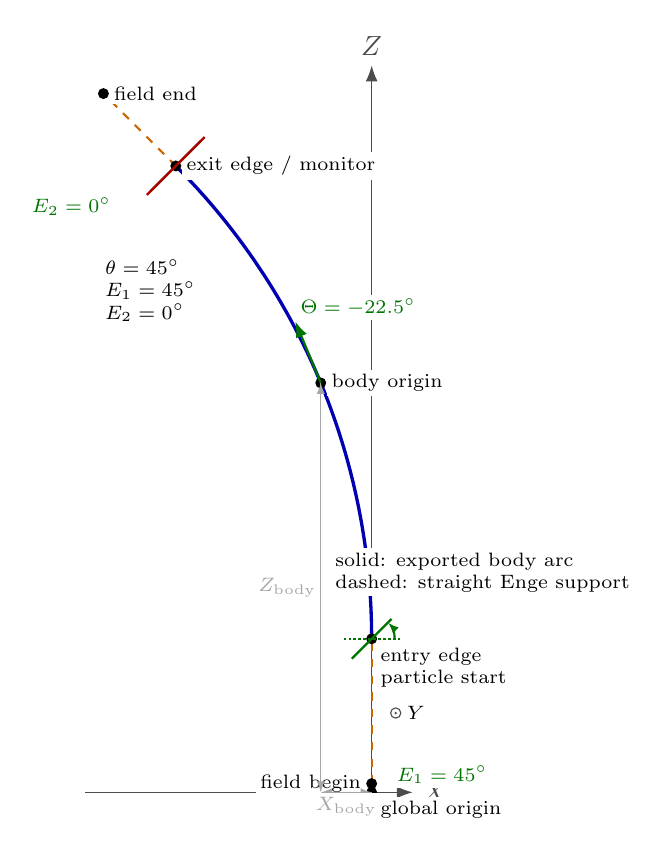
\begin{tikzpicture}[x=6.5cm,y=6.5cm]
  \def\h{0.7653668647301796}
  \def\hdeg{43.85229112819947}
  \def\Xb{-0.0994561837}
  \def\Zb{0.8000000000}
  \def\Tb{-22.5}

  \coordinate (O) at (0,0);

  \draw[axis] (-0.56,0) -- (0.08,0) node[right] {$X$};
  \draw[axis] (0,-0.04) -- (0,1.42) node[above] {$Z$};
  \node[marker,label={[note]below right:global origin}] at (O) {};
  \draw[black!70] (0.047,0.155) circle (0.010);
  \fill[black!70] (0.047,0.155) circle (0.0025);
  \node[note,anchor=west] at (0.060,0.155) {$Y$};

  \draw[design]
    plot[domain=-0.5130860765:0.5130860765,samples=90,variable=\s]
    ({\Xb + cos(\Tb)*((cos(\hdeg*\s)-1)/\h) + sin(\Tb)*(sin(\hdeg*\s)/\h)},
     {\Zb - sin(\Tb)*((cos(\hdeg*\s)-1)/\h) + cos(\Tb)*(sin(\hdeg*\s)/\h)});

  \coordinate (FB) at (0.0000000000,0.0171572875);
  \coordinate (EN) at (0.0000000000,0.3000000000);
  \coordinate (BO) at (-0.0994561837,0.8000000000);
  \coordinate (EX) at (-0.3826834324,1.2238795325);
  \coordinate (FE) at (-0.5241047886,1.3653008887);
  \coordinate (MO) at (-0.3826834324,1.2238795325);

  \draw[fringe] (FB) -- (EN);
  \draw[fringe] (EX) -- (FE);

  \node[marker,label={[note]left:field begin}] at (FB) {};
  \node[marker,label={[note]below right:entry edge\\particle start}] at (EN) {};
  \node[marker,label={[note]right:body origin}] at (BO) {};
  \node[marker,label={[note]right:exit edge / monitor}] at (EX) {};
  \node[marker,label={[note]right:field end}] at (FE) {};

  \draw[gray!70,densely dashed] (O) -- (\Xb,0) -- (BO);
  \draw[{Latex[length=1.4mm]}-{Latex[length=1.4mm]}, gray!70] (O) -- (\Xb,0)
    node[midway,below,note] {$X_\mathrm{body}$};
  \draw[{Latex[length=1.4mm]}-{Latex[length=1.4mm]}, gray!70] (\Xb,0) -- (BO)
    node[midway,left,note] {$Z_\mathrm{body}$};

  \draw[pose] (BO) -- ++({0.13*sin(\Tb)},{0.13*cos(\Tb)})
    node[note,above right] {$\Theta=-22.5\degree$};

  \draw[poleface,densely dotted] ($(EN)+(-0.055,0)$) -- ($(EN)+(0.055,0)$);
  \draw[poleface]
    ($(EN)+({-0.055*cos(45)},{-0.055*sin(45)})$) --
    ($(EN)+({0.055*cos(45)},{0.055*sin(45)})$);
  \draw[poleangle] ($(EN)+(0.045,0)$)
    arc[start angle=0,end angle=45,radius=0.045];
  \node[note,text=green!45!black,anchor=west] at (0.040,0.034)
    {$E_1=45\degree$};

  \draw[poleface]
    ($(EX)+({-0.070*cos(45)},{-0.070*sin(45)})$) --
    ($(EX)+({0.070*cos(45)},{0.070*sin(45)})$);
  \node[note,text=green!45!black,anchor=east] at (-0.500,1.145)
    {$E_2=0\degree$};

  \draw[monitor] (MO) -- ++({0.08*cos(-45)},{-0.08*sin(-45)});
  \draw[monitor] (MO) -- ++({-0.08*cos(-45)},{0.08*sin(-45)});

  \node[note,anchor=west] at (-0.53,0.98)
    {$\theta=45\degree$\\$E_1=45\degree$\\$E_2=0\degree$};
  \node[note,anchor=west] at (-0.08,0.43)
    {solid: exported body arc\\dashed: straight Enge support};
\end{tikzpicture}
\caption{\code{test-sbend-1}: placed body arc, field support, and temporal monitor plane.
The grey dimensions mark the OPALX body pose in the global \(X\)-\(Z\) projection;
the circled-dot axis marks global \(+Y\) normal to the page.  The entrance
pole face is \(45\degree\), but the on-axis start particle remains on the
design exit.}
\end{figure}

\section{\code{test-sbend-1}: OPAL 2022.1 comparison}

The old-OPAL comparison uses \code{test-sbend-1\_opal.in} with the same
\code{SBEND} length, angle, pole-face angles, gap, and fringe integral.  The
comparison script runs OPALX and OPAL 2022.1 in separate work directories and
compares only the \code{DesignPath.dat} and \code{.stat} diagnostics; HDF5 and
load-balance files are ignored.

In the 30 cm drift comparison used for these figures, the reference-particle
\(B_y\) peak agrees exactly at the sampled precision.  The \code{.stat}
reference-field support starts at the same longitudinal coordinate and ends
within \(3\times 10^{-4}\ \mathrm{m}\).  The remaining path differences are
small compared with the bend scale: the maximum design-path differences are
\(4.4\times10^{-4}\ \mathrm{m}\) in \(x\) and
\(2.1\times10^{-4}\ \mathrm{m}\) in relative \(z\).

\begin{figure}[htbp]
\centering
\begin{minipage}{0.49\textwidth}
\centering
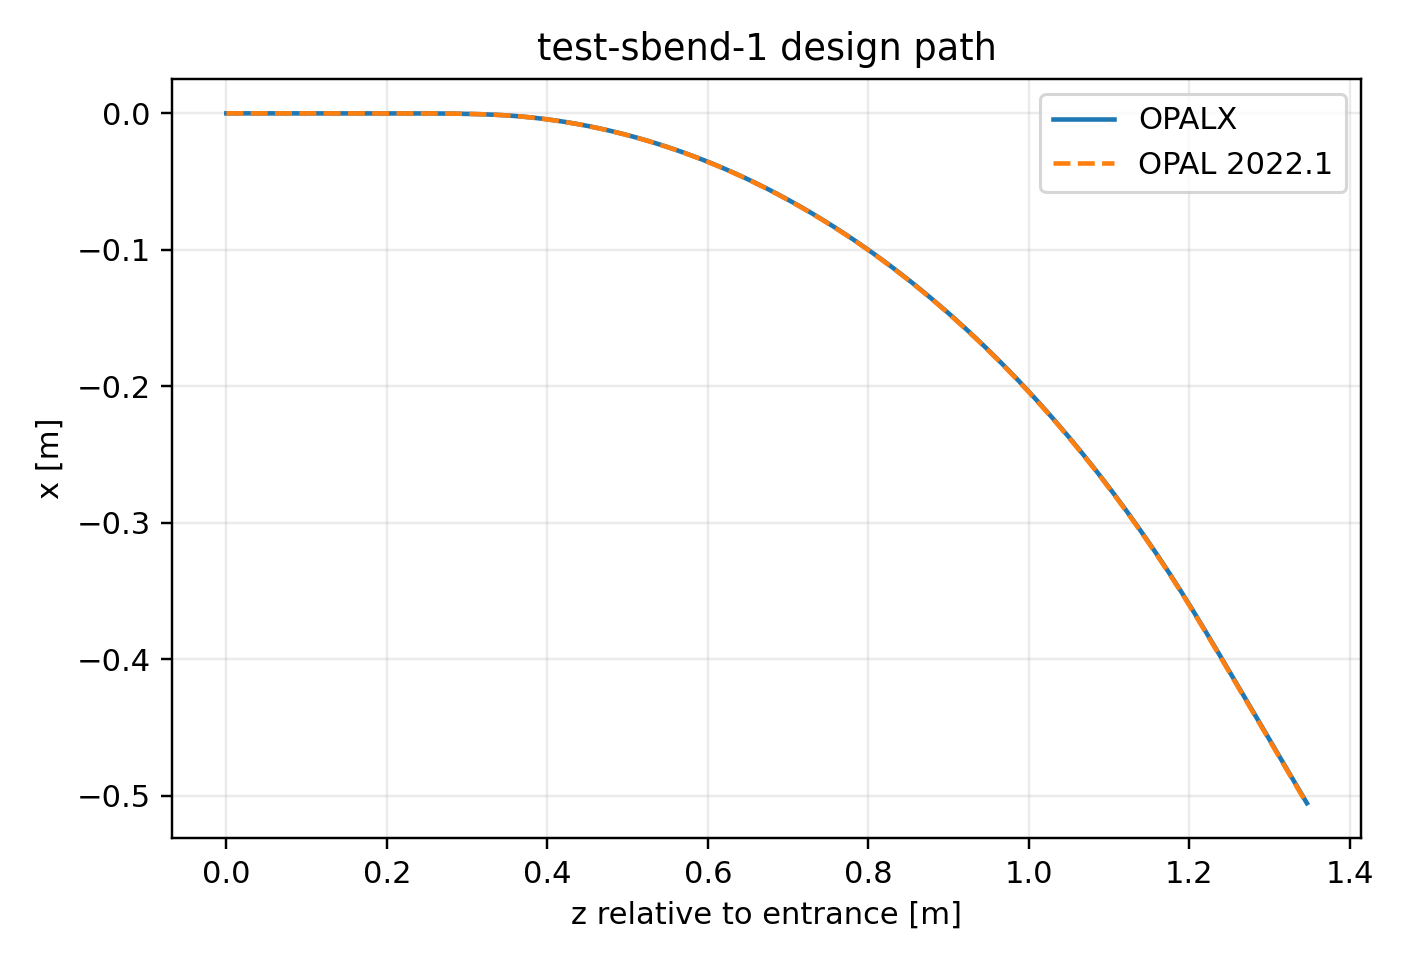
\includegraphics[width=\linewidth]{figures/test-sbend-1-design-path-xz.png}
\end{minipage}\hfill
\begin{minipage}{0.49\textwidth}
\centering
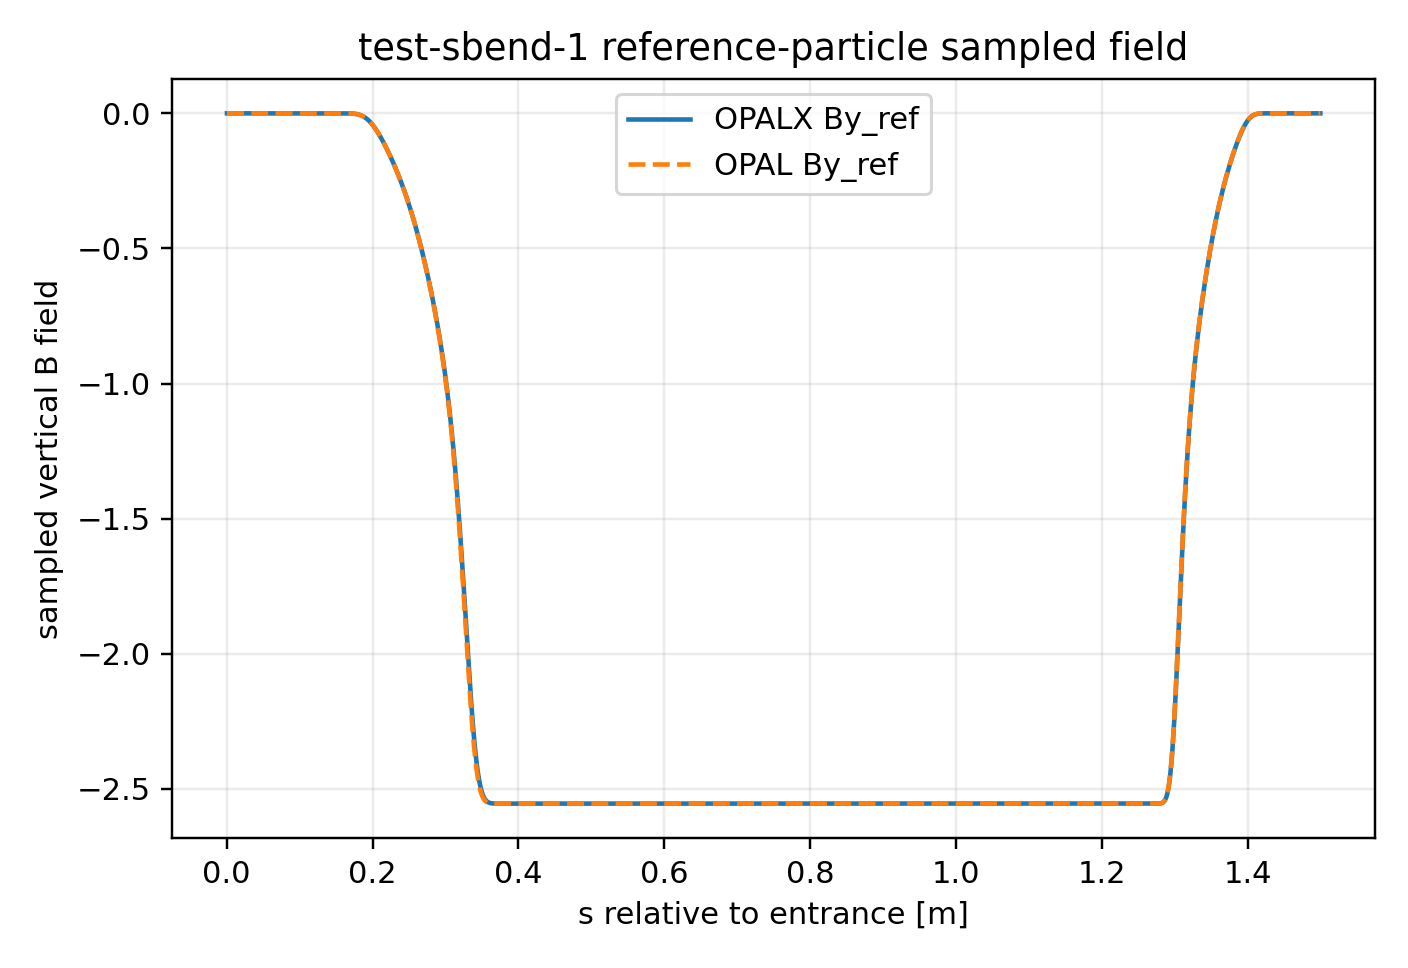
\includegraphics[width=\linewidth]{figures/test-sbend-1-stat-by-ref.png}
\end{minipage}
\caption{\code{test-sbend-1} OPALX versus OPAL 2022.1: design-path
\(X\)-\(Z\) orbit (left) and \code{.stat} reference \(B_y\) (right).}
\end{figure}

\begin{figure}[htbp]
\centering
\begin{minipage}{0.49\textwidth}
\centering
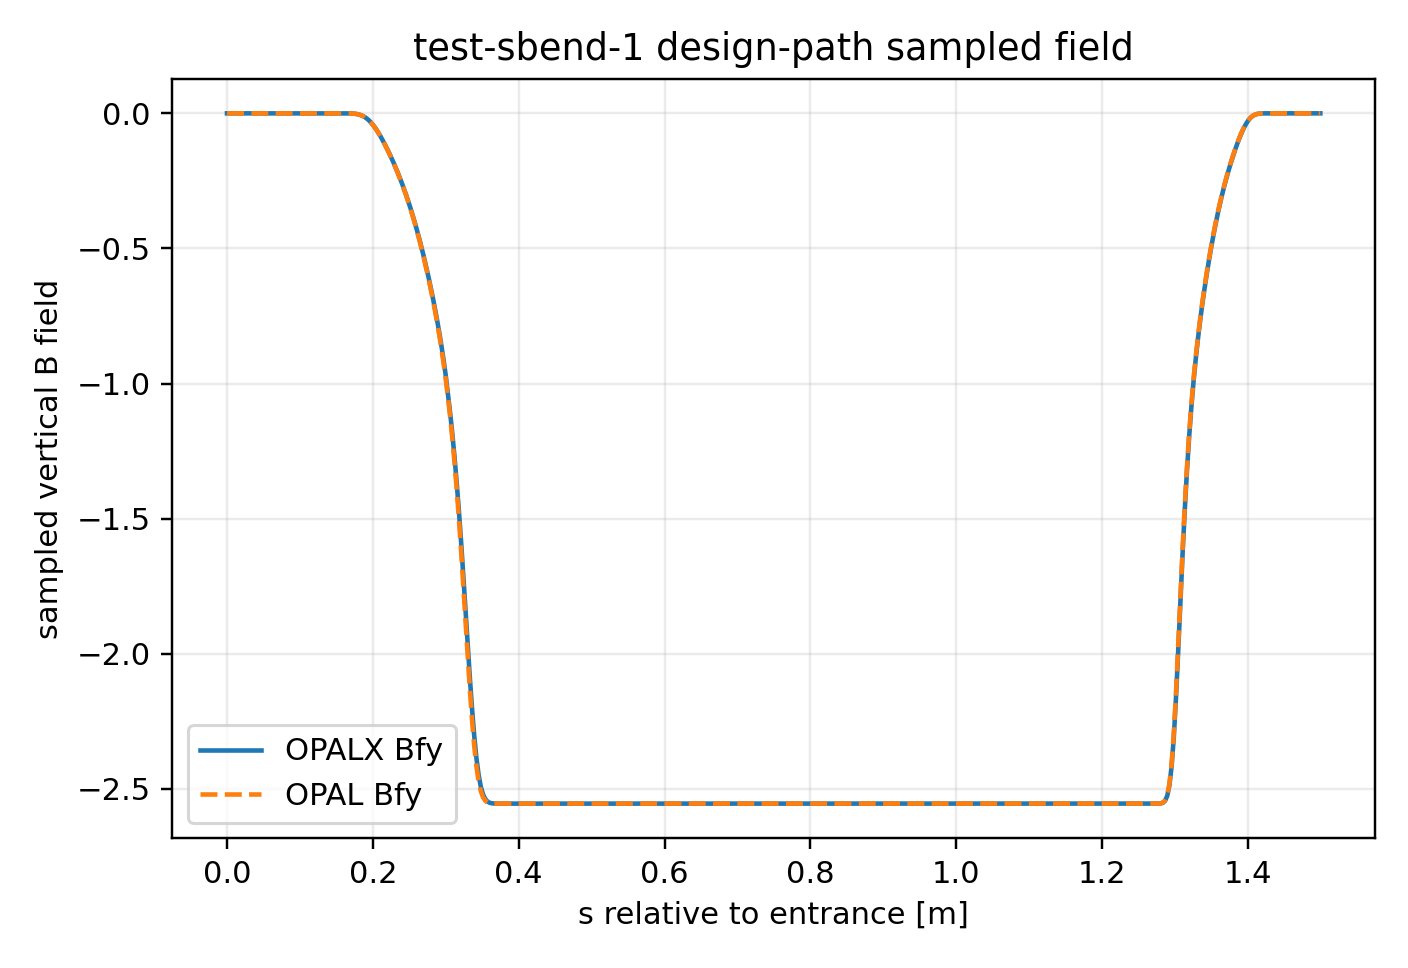
\includegraphics[width=\linewidth]{figures/test-sbend-1-design-path-by.png}
\end{minipage}\hfill
\begin{minipage}{0.49\textwidth}
\centering
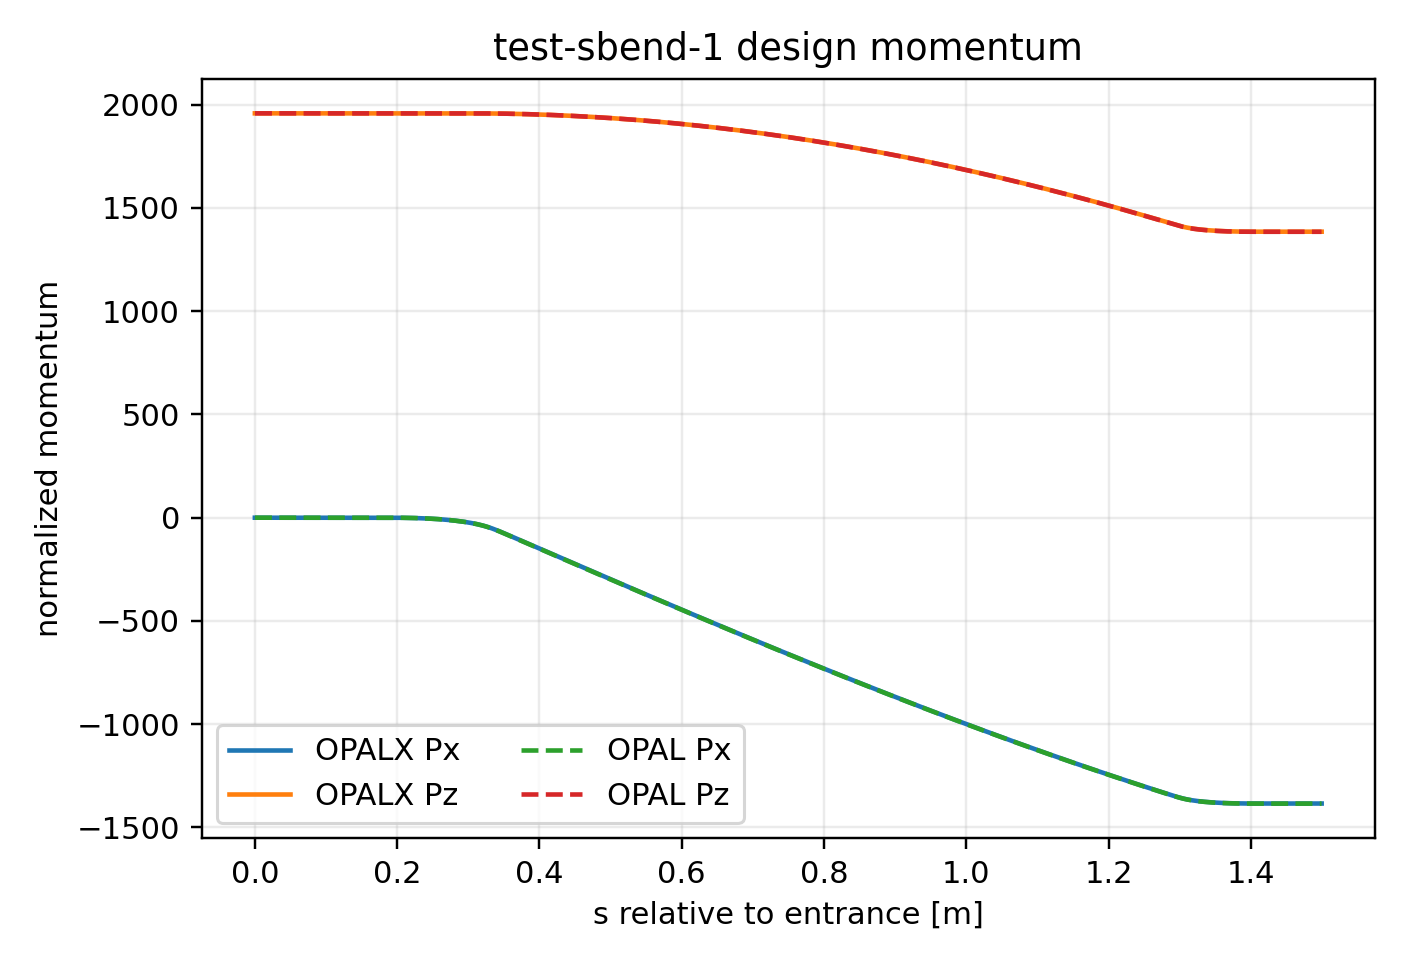
\includegraphics[width=\linewidth]{figures/test-sbend-1-design-path-momentum.png}
\end{minipage}
\caption{\code{test-sbend-1} design-path diagnostic comparison.  Left: sampled
\(B_y\) from \code{DesignPath.dat}.  Right: design-path momentum components.}
\end{figure}

\section{\code{test-sbend-2}: OPALX/OPAL vertical edge-focusing comparison}

This test keeps the same chord-to-arc SBEND placement formulas as
\code{test-sbend-1}, but launches a particle with
\[
  y_0 = 1.0\ \mathrm{mm},\qquad y'_0 = 0.
\]
The OPALX input is \code{sandbox/test-sbend-2/test-sbend-2.in}; the old OPAL
reference input is \code{sandbox/test-sbend-2/test-sbend-2\_opal.in}.  OPALX
uses explicit element placement, while old OPAL uses \code{ELEMEDGE}.  The old
OPAL distribution is replicated to \(10^4\) identical macro-particles so that
OPAL 2022.1 writes the standard \code{.stat} diagnostics; OPALX uses a single
particle and no self field.

\begin{center}
\begin{tabular}{@{}ll@{}}
\toprule
quantity & value \\
\midrule
upstream drift & \(0.4\ \mathrm{m}\) \\
\code{ANGLE} & \(45\degree\) \\
\code{E1}, \code{E2} & \(-49.99\degree,\ 0\degree\) \\
\code{HGAP}, \code{FINT} & \(0.02\ \mathrm{m},\ 0.5\) \\
OPAL full \code{GAP} & \(0.04\ \mathrm{m}\) \\
Enge half width \(a=5\,\code{GAP}\) & \(0.2\ \mathrm{m}\) \\
\(\ell_\mathrm{entry}=a/|\cos E_1|\) & \(0.3110798769\ \mathrm{m}\) \\
\(\ell_\mathrm{exit}=a/\cos E_2\) & \(0.2\ \mathrm{m}\) \\
upstream Enge support start & \(0.0889199346\ \mathrm{m}\) \\
nominal entrance edge & \(0.4\ \mathrm{m}\) \\
nominal exit edge & \(1.4261721530\ \mathrm{m}\) \\
\bottomrule
\end{tabular}
\end{center}

The comparison run uses
\[
  s_\mathrm{rel}^{\mathrm{OPAL}} = s^{\mathrm{OPAL}} - 1\ \mathrm{m},
  \qquad
  z_\mathrm{rel}^{\mathrm{OPAL}} = z^{\mathrm{OPAL}} - 1\ \mathrm{m}.
\]
The apparent bend start near \(0.2\ \mathrm{m}\) is not a different OPALX
element placement.  It is the visible part of the upstream Enge fringe.  The
full OPAL-style support begins at \(0.4-\ell_\mathrm{entry}
=0.0889199346\ \mathrm{m}\), where the field is still numerically tiny, and
the nominal bend entrance remains at \(0.4\ \mathrm{m}\) in both OPALX and old
OPAL.  With the comparison script's \(10^{-6}\) peak-field support threshold,
the design-path \(B_y\) fringe starts at \(0.2401337\ \mathrm{m}\) in OPALX
and \(0.2399838\ \mathrm{m}\) in old OPAL.

The reference geometry and field profile agree at the same level as the
placement test: \(B_y\) peak differences are zero in the sampled output, the
design-path \(B_y\) integral differs by \(1.21\times 10^{-3}\), and the
\code{.stat} reference-particle field support ends within \(6.0\times 10^{-4}\)
m.  The OPALX vertical edge force is now weighted with the same Enge
derivative as the fringe field, so the equivalent kick is applied at the same
longitudinal centroid as old OPAL's map.  At the final common sample OPALX has
\(\bar y=2.168074\times 10^{-3}\ \mathrm{m}\), while old OPAL has
\(\bar y=2.161588\times 10^{-3}\ \mathrm{m}\).  The remaining final difference
is \(6.49\times 10^{-6}\ \mathrm{m}\), so this case is now a useful
vertical-focusing regression diagnostic.

\begin{figure}[htbp]
\centering
\begin{minipage}{0.49\textwidth}
\centering
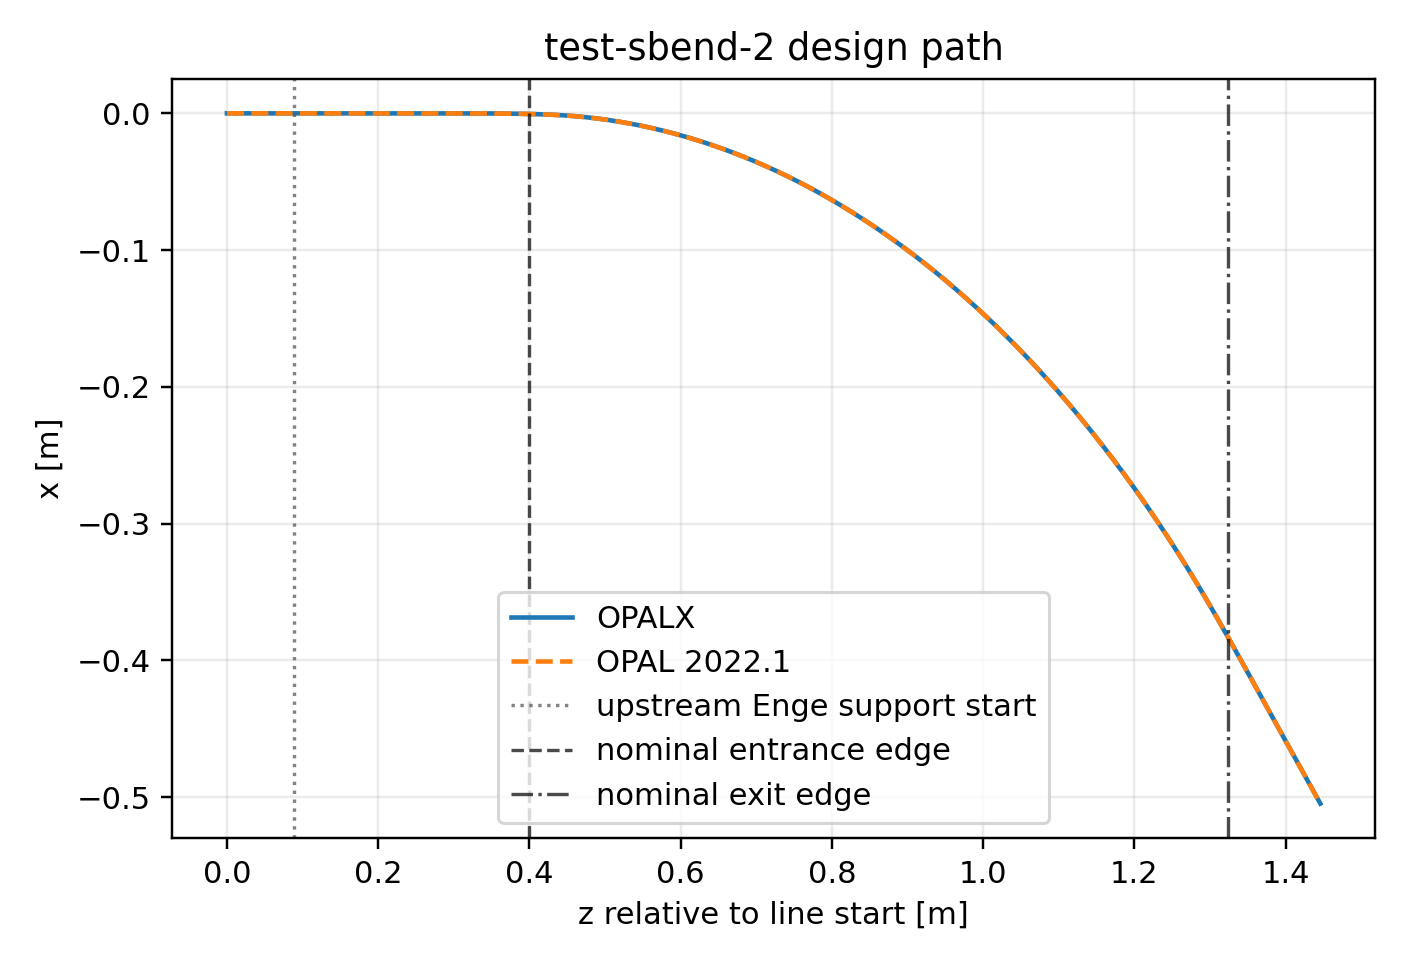
\includegraphics[width=\linewidth]{figures/test-sbend-2-design-path-xz.png}
\end{minipage}\hfill
\begin{minipage}{0.49\textwidth}
\centering
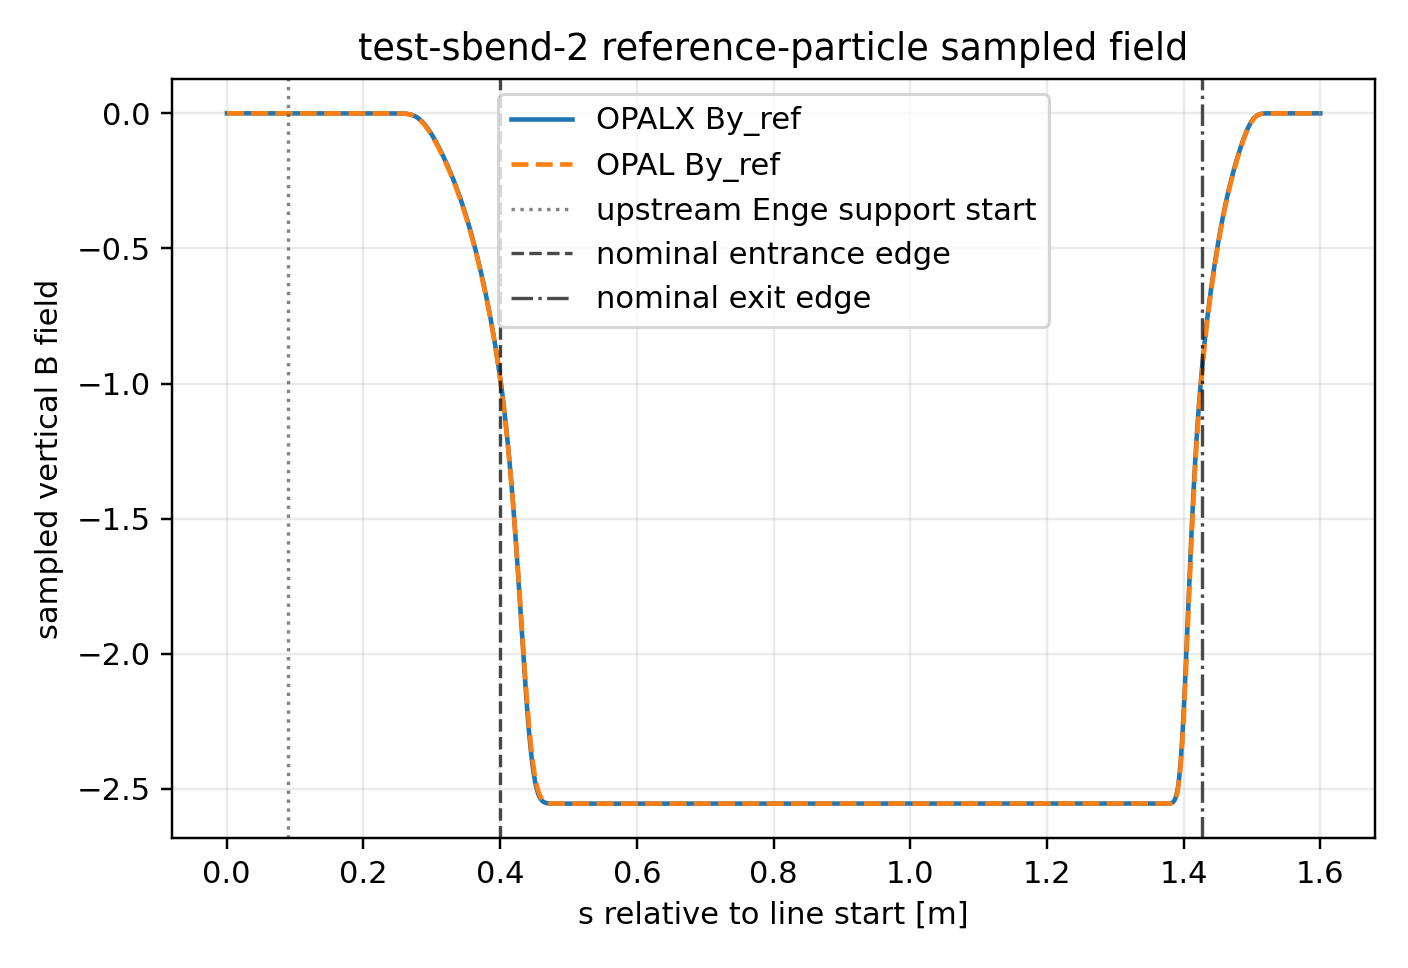
\includegraphics[width=\linewidth]{figures/test-sbend-2-stat-by-ref.png}
\end{minipage}
\caption{\code{test-sbend-2} OPALX versus OPAL 2022.1: design-path
\(X\)-\(Z\) orbit (left) and \code{.stat} reference \(B_y\) (right).  The
dotted vertical marker is the upstream Enge support start; dashed and
dash-dotted markers are the nominal entrance and exit edges.}
\end{figure}

\begin{figure}[htbp]
\centering
\begin{minipage}{0.49\textwidth}
\centering
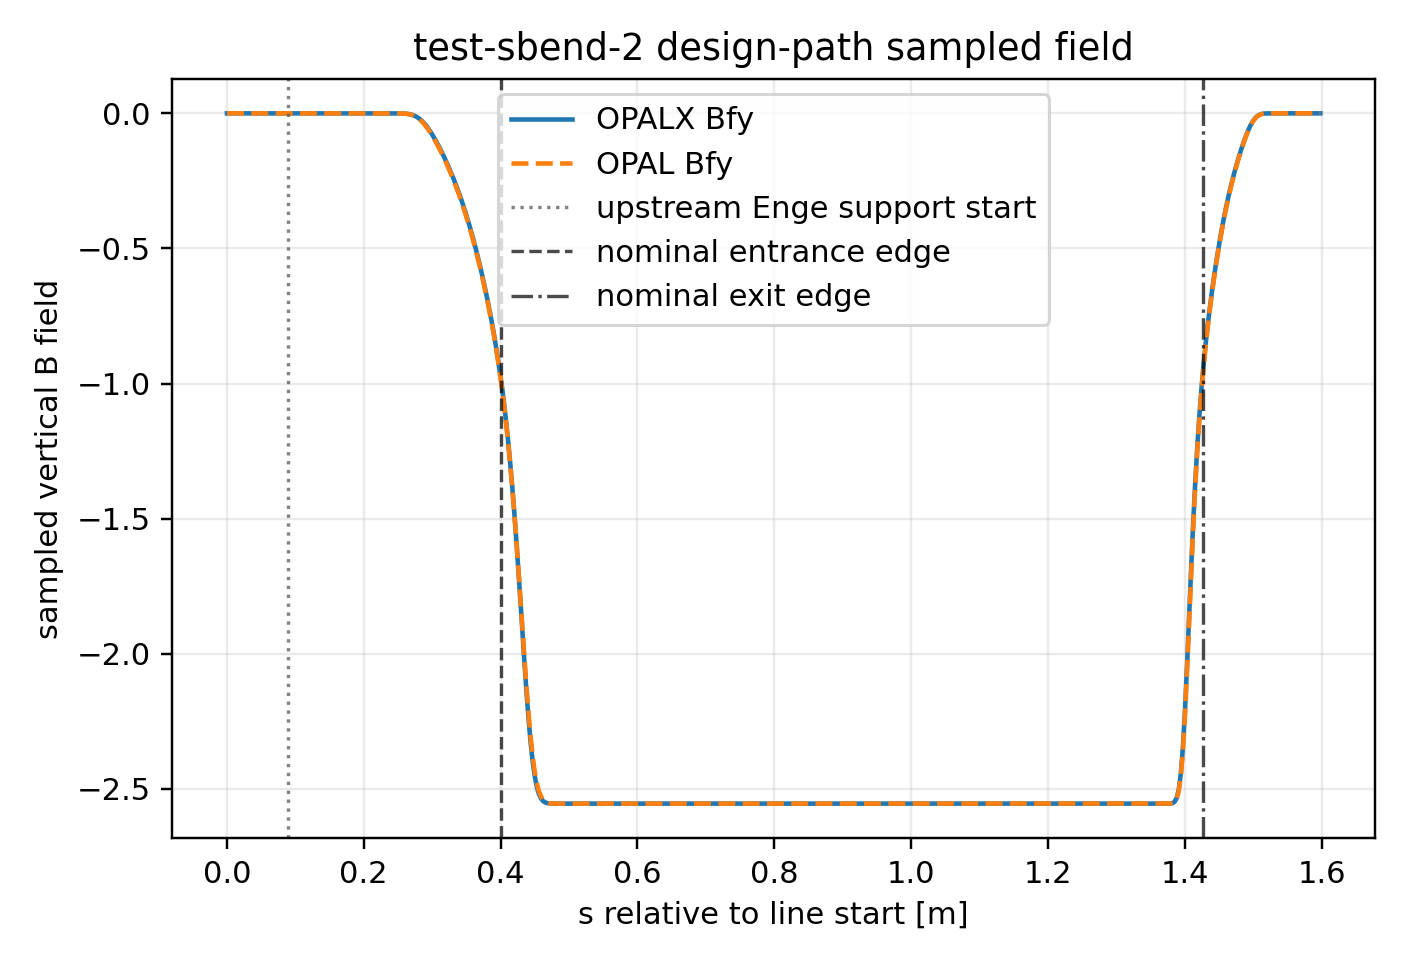
\includegraphics[width=\linewidth]{figures/test-sbend-2-design-path-by.png}
\end{minipage}\hfill
\begin{minipage}{0.49\textwidth}
\centering
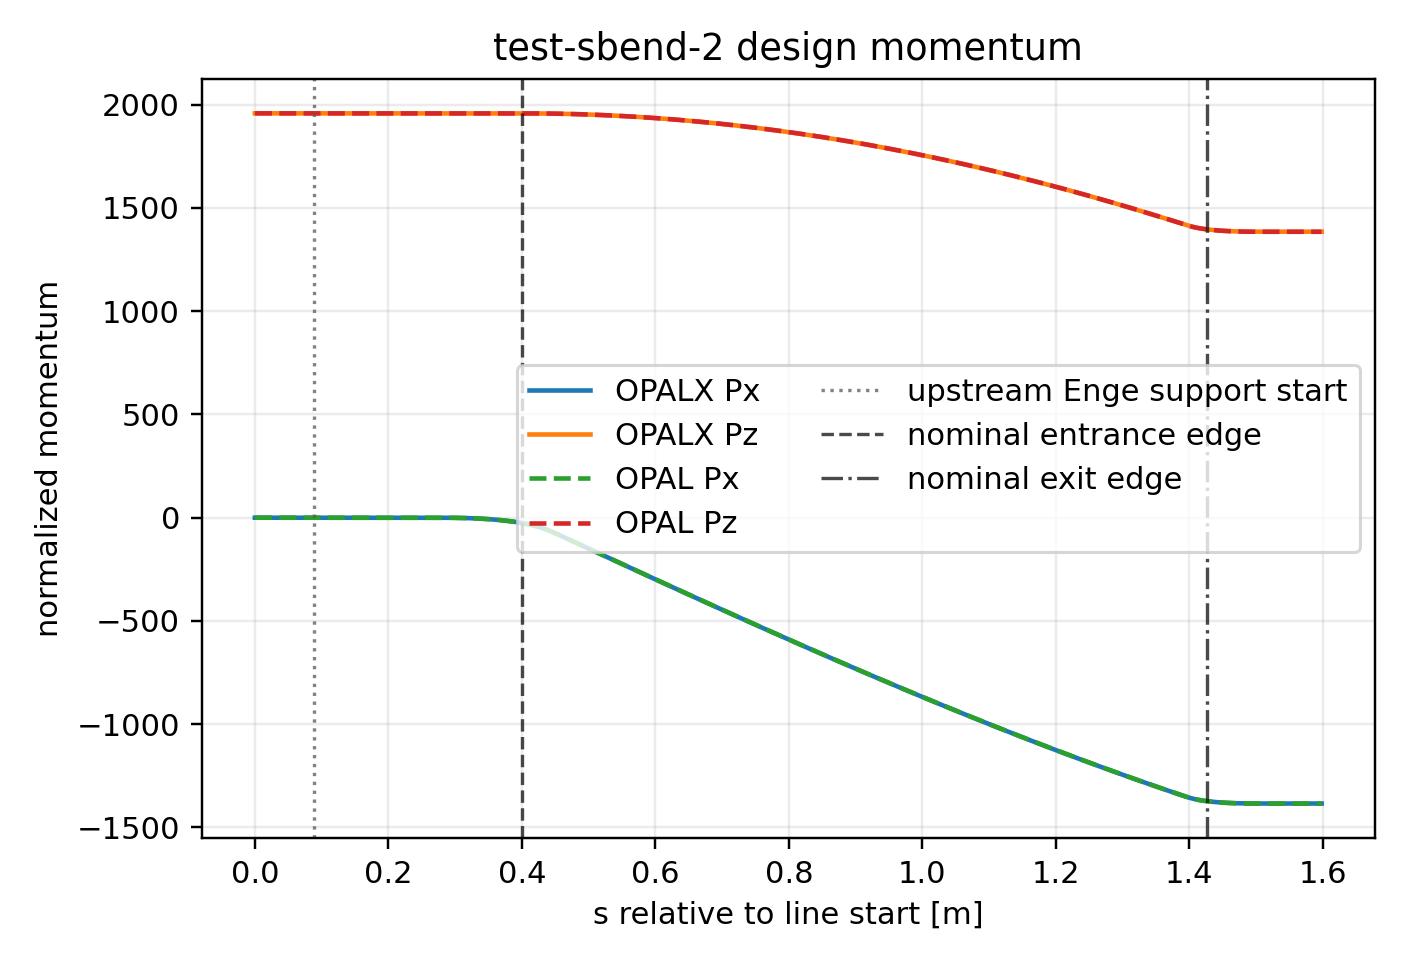
\includegraphics[width=\linewidth]{figures/test-sbend-2-design-path-momentum.png}
\end{minipage}
\caption{\code{test-sbend-2} design-path diagnostic comparison.  Left: sampled
\(B_y\) from \code{DesignPath.dat}.  Right: design-path momentum components.
The same geometry markers show that the visible fringe precedes the nominal
\(0.4\ \mathrm{m}\) entrance edge in both codes.}
\end{figure}

\begin{figure}[htbp]
\centering
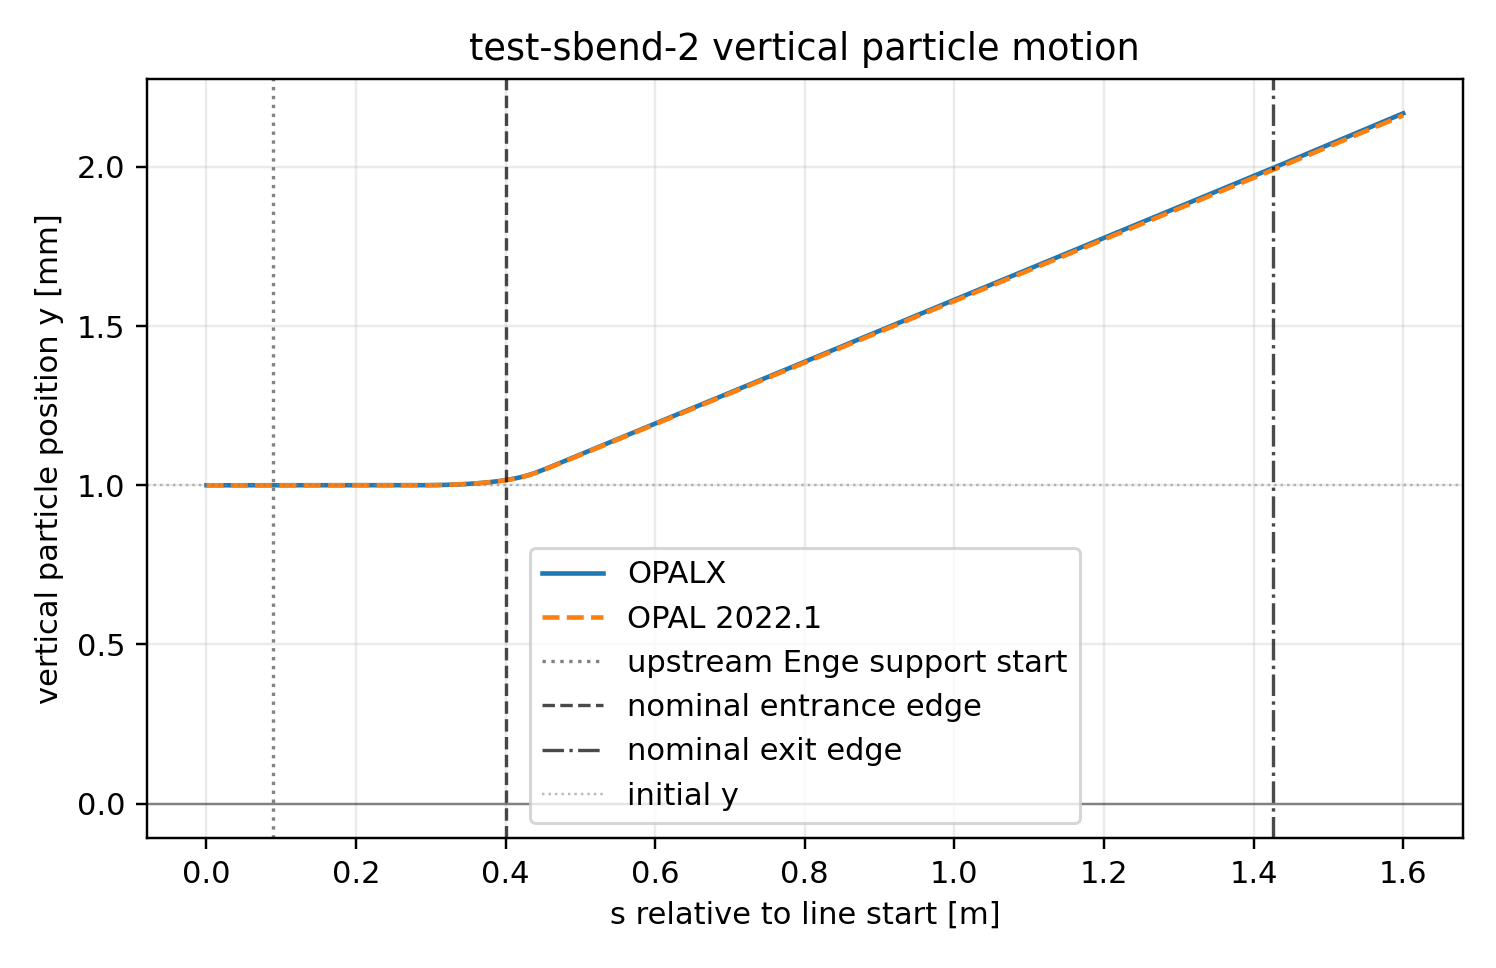
\includegraphics[width=0.78\linewidth]{figures/test-sbend-2-vertical-particle-motion.png}
\caption{\code{test-sbend-2} vertical particle motion from the \code{.stat}
\(\bar y\) column.  Both distributions are monoenergetic replicated particles,
so \(\bar y\) is the tracked particle's vertical coordinate.}
\end{figure}

\section{\code{test-rbend-1}: placement consistency test}

This test is the RBEND analogue of \code{test-sbend-1}: a single on-axis
particle, a \(0.3\ \mathrm{m}\) upstream drift, and an explicit \code{RBEND}
body pose derived from the formulas above.  The input decks are
\[
  \code{sandbox/test-rbend-1/test-rbend-1.in},\qquad
  \code{sandbox/test-rbend-1/test-rbend-1\_opal.in}.
\]
The exported OPALX element positions confirm the requested rectangular
geometry:

\begin{center}
\begin{tabular}{@{}ll@{}}
\toprule
quantity & OPALX export \\
\midrule
entrance edge & \(X=5.6\times10^{-17},\ Z=0.3000000000\ \mathrm{m}\) \\
body pose & \(X=0.2832272487,\ Z=-0.1238795325,\ \Theta=-22.5\degree\) \\
exit edge & \(X=-0.4142135624,\ Z=1.3000000000\ \mathrm{m}\) \\
field support & \(Z=0.1\) to \(1.609014865\ \mathrm{m}\) \\
\bottomrule
\end{tabular}
\end{center}

The placement export is therefore consistent with the analytic rectangular
survey.  With the RBEND field evaluated in the OPAL-compatible rectangular edge
frames and normalized with \(R_\mathrm{CH}\), the physics comparison is now at
the same level as the SBEND checks.  In the \code{DesignPath.dat} comparison
the largest orbit differences are \(2.22\times10^{-5}\ \mathrm{m}\) in \(X\)
and \(2.28\times10^{-5}\ \mathrm{m}\) in relative \(Z\).  The sampled \(B_y\)
peaks are \(2.3598578\) in OPALX and \(2.3598593\) in OPAL, and the
design-path \(B_y\) integral differs by \(4.35\times10^{-4}\).  The
\code{.stat} reference-particle field support ends within
\(3.0\times10^{-4}\ \mathrm{m}\).

\begin{figure}[htbp]
\centering
\begin{minipage}{0.49\textwidth}
\centering
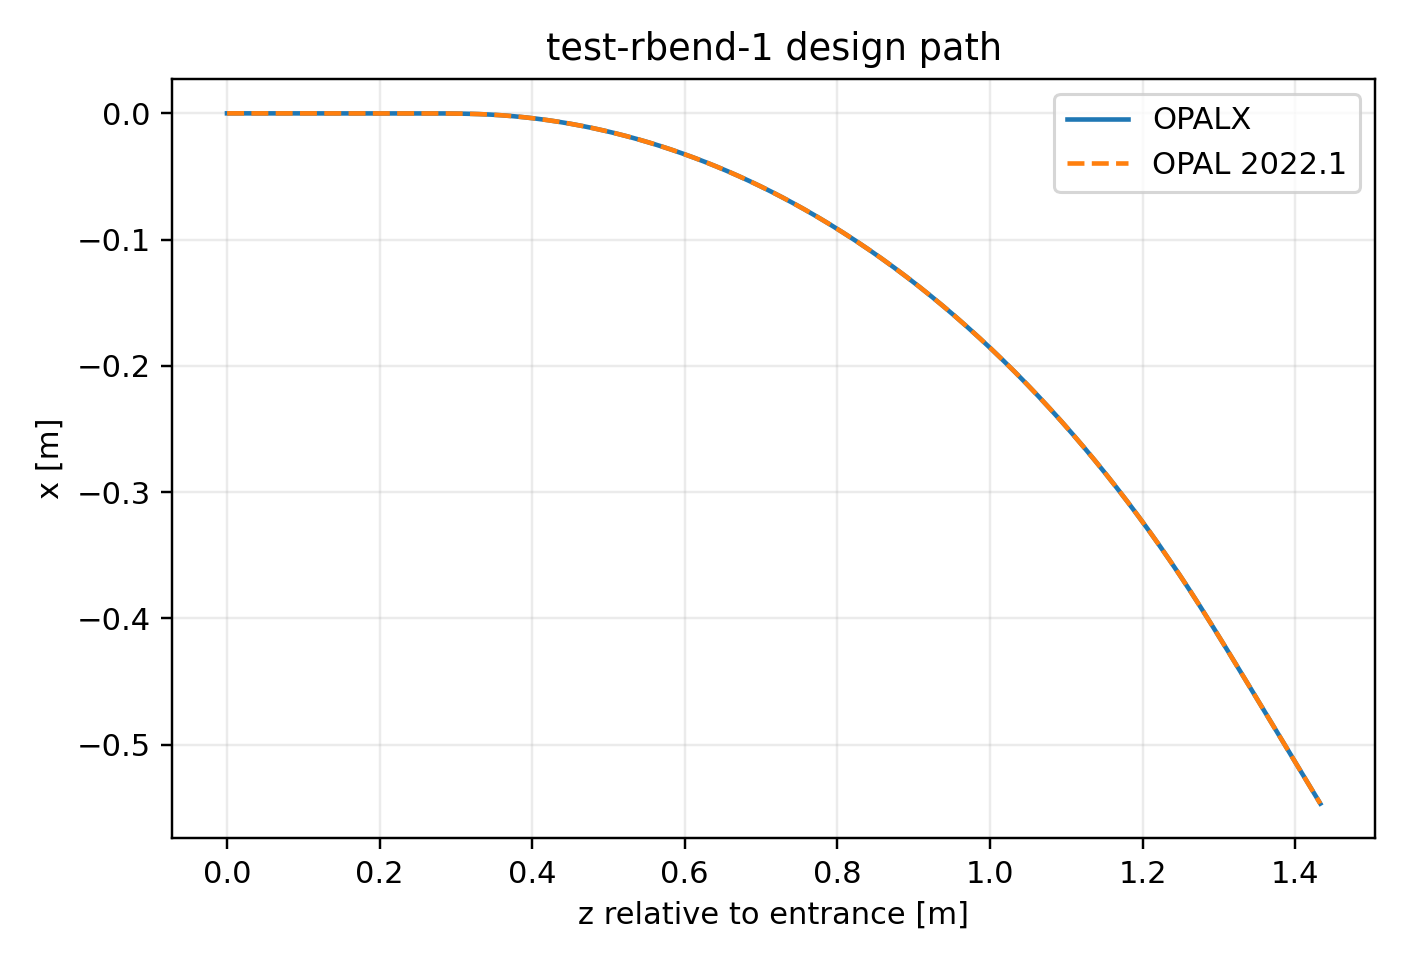
\includegraphics[width=\linewidth]{figures/test-rbend-1-design-path-xz.png}
\end{minipage}\hfill
\begin{minipage}{0.49\textwidth}
\centering
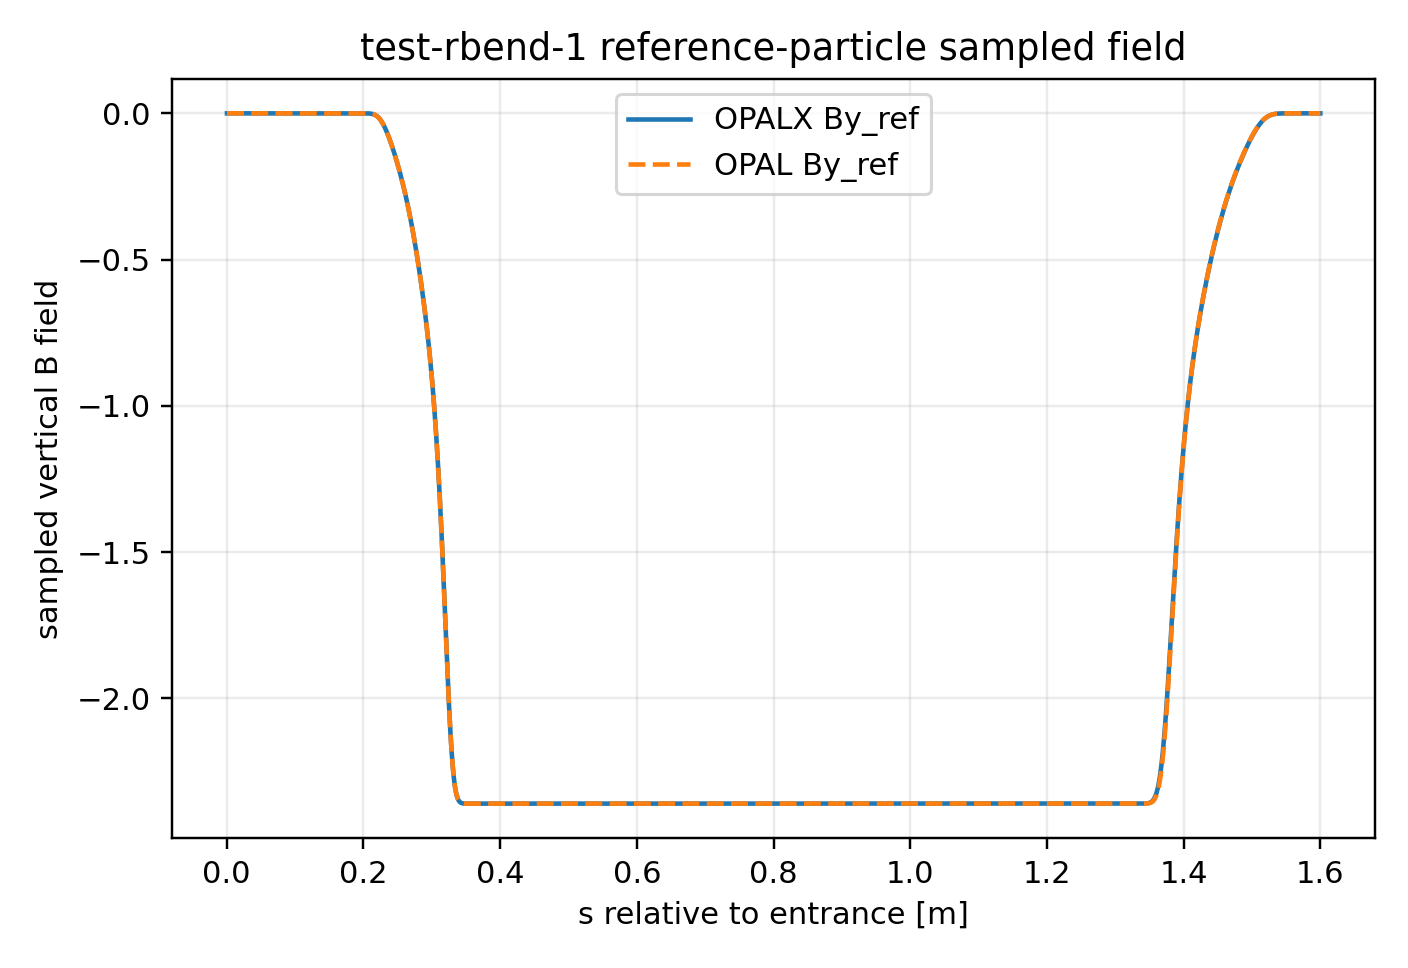
\includegraphics[width=\linewidth]{figures/test-rbend-1-stat-by-ref.png}
\end{minipage}
\caption{\code{test-rbend-1} OPALX versus OPAL 2022.1: design-path
\(X\)-\(Z\) orbit (left) and \code{.stat} reference \(B_y\) (right).}
\end{figure}

\begin{figure}[htbp]
\centering
\begin{minipage}{0.49\textwidth}
\centering
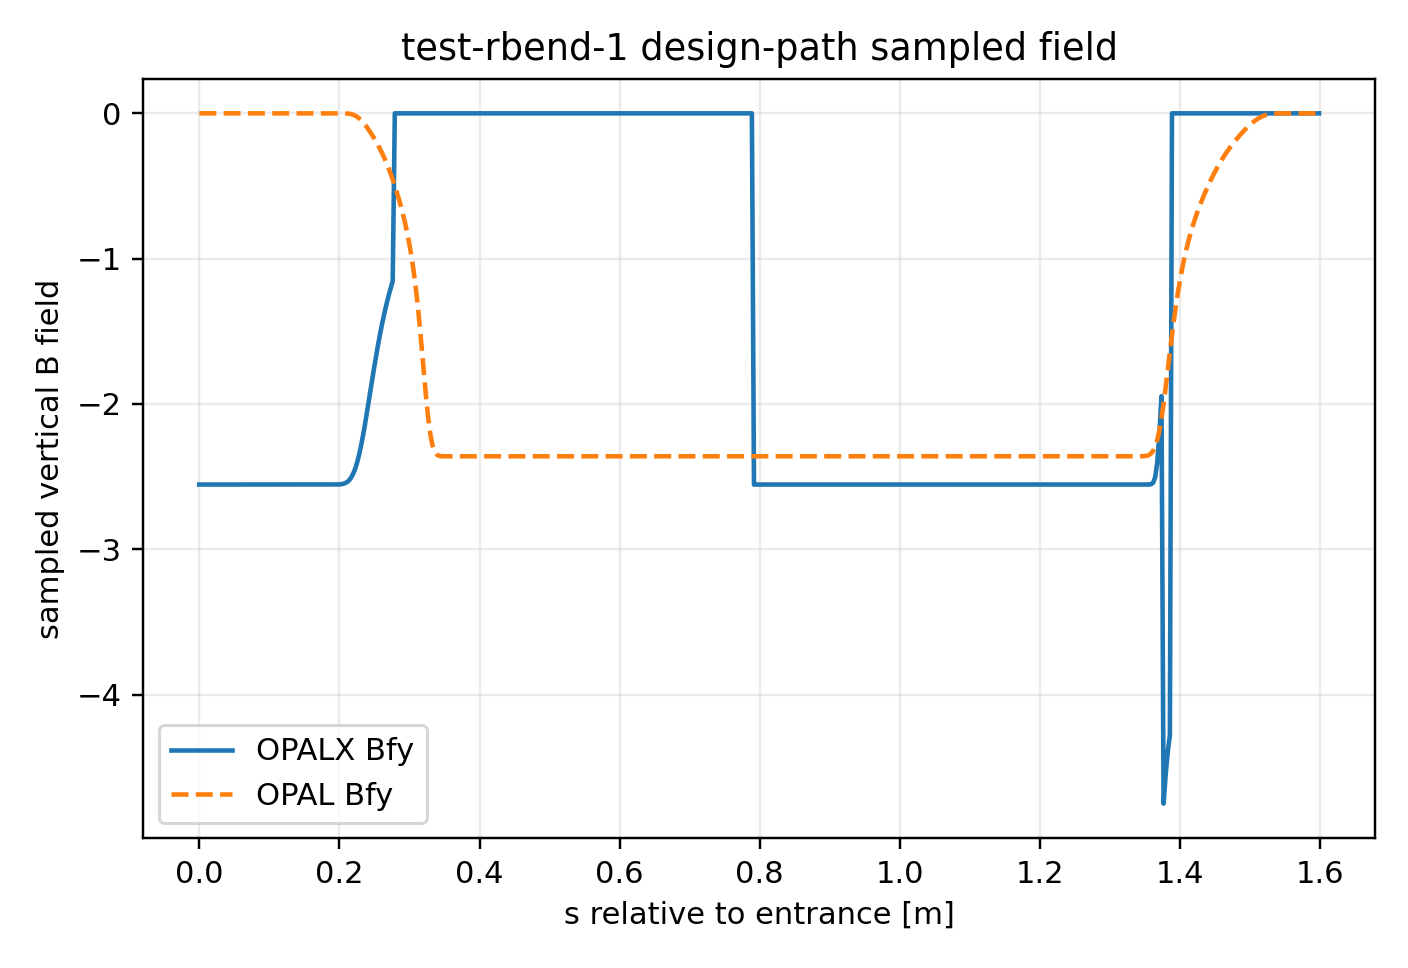
\includegraphics[width=\linewidth]{figures/test-rbend-1-design-path-by.png}
\end{minipage}\hfill
\begin{minipage}{0.49\textwidth}
\centering
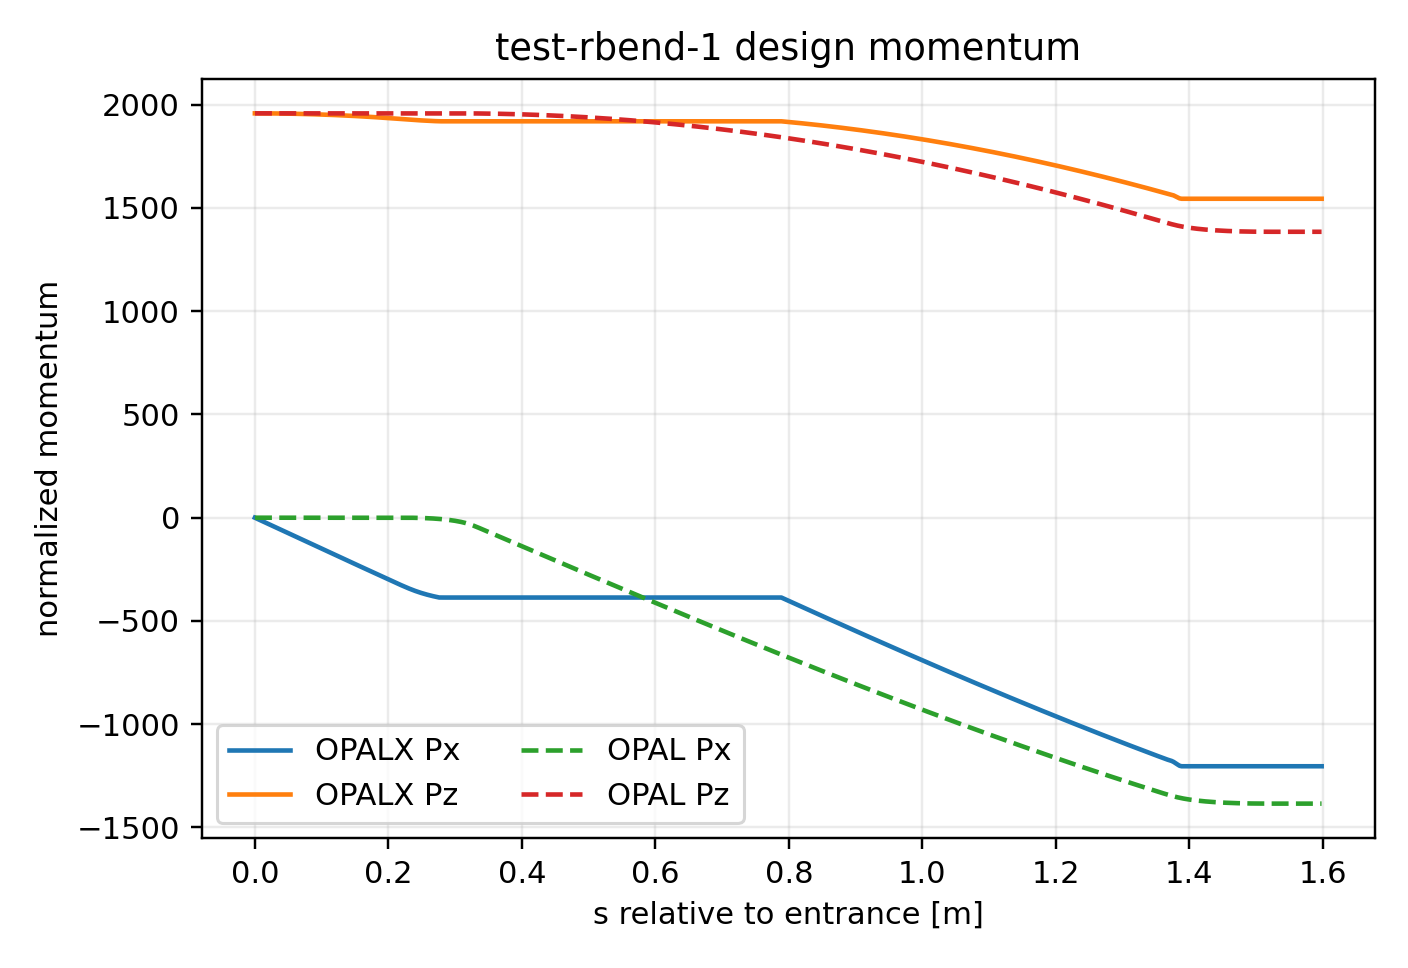
\includegraphics[width=\linewidth]{figures/test-rbend-1-design-path-momentum.png}
\end{minipage}
\caption{\code{test-rbend-1} design-path diagnostic comparison.  The RBEND
\(B_y\) peak and longitudinal support now match old OPAL at the sampled
precision needed for the placement regression.}
\end{figure}

\section{\code{test-rbend-2}: OPALX/OPAL vertical comparison}

This test is the RBEND counterpart of \code{test-sbend-2}.  It uses a
\(0.4\ \mathrm{m}\) upstream drift and launches the particle with
\[
  y_0=1.0\ \mathrm{mm},\qquad y'_0=0.
\]
The OPALX input is \code{sandbox/test-rbend-2/test-rbend-2.in}; the old OPAL
reference input is \code{sandbox/test-rbend-2/test-rbend-2\_opal.in}.  The
same rectangular formulas give
\[
\begin{aligned}
  \vect r_\mathrm{entry} &= (0,\,0,\,0.4000000000)\ \mathrm{m},\\
  \vect r_\mathrm{body}  &= (0.2832272487,\,0,\,-0.0238795325)\ \mathrm{m},\\
  \vect r_\mathrm{exit}  &= (-0.4142135624,\,0,\,1.4000000000)\ \mathrm{m}.
\end{aligned}
\]
The comparison markers are
\[
\begin{array}{@{}lll@{}}
\text{upstream Enge support start} & s_\mathrm{rel}=0.2000000 & z_\mathrm{rel}=0.2000000,\\
\text{nominal entrance edge}       & s_\mathrm{rel}=0.4000000 & z_\mathrm{rel}=0.4000000,\\
\text{nominal exit edge}           & s_\mathrm{rel}=1.5107207 & z_\mathrm{rel}=1.4000000,\\
\text{downstream support end}      & s_\mathrm{rel}=1.7935634 & z_\mathrm{rel}=1.6000000 .
\end{array}
\]

The RBEND vertical test now provides a clean edge-focusing regression.  The
\code{DesignPath.dat} \(B_y\) peaks are \(2.3598578\) in OPALX and
\(2.3598593\) in OPAL; the design-path \(B_y\) integral differs by
\(4.35\times10^{-4}\), and the visible field support starts and ends within
\(1.5\times10^{-4}\ \mathrm{m}\).  At the final common \code{.stat} sample the
mean vertical positions are
\[
  \bar y_\mathrm{OPALX}=8.817085\times10^{-4}\ \mathrm{m},\qquad
  \bar y_\mathrm{OPAL}=8.804121\times10^{-4}\ \mathrm{m},
\]
for a final difference of \(1.30\times10^{-6}\ \mathrm{m}\).  This makes the
case suitable as the RBEND counterpart of the \code{test-sbend-2} vertical
edge-focusing regression.

\begin{figure}[htbp]
\centering
\begin{minipage}{0.49\textwidth}
\centering
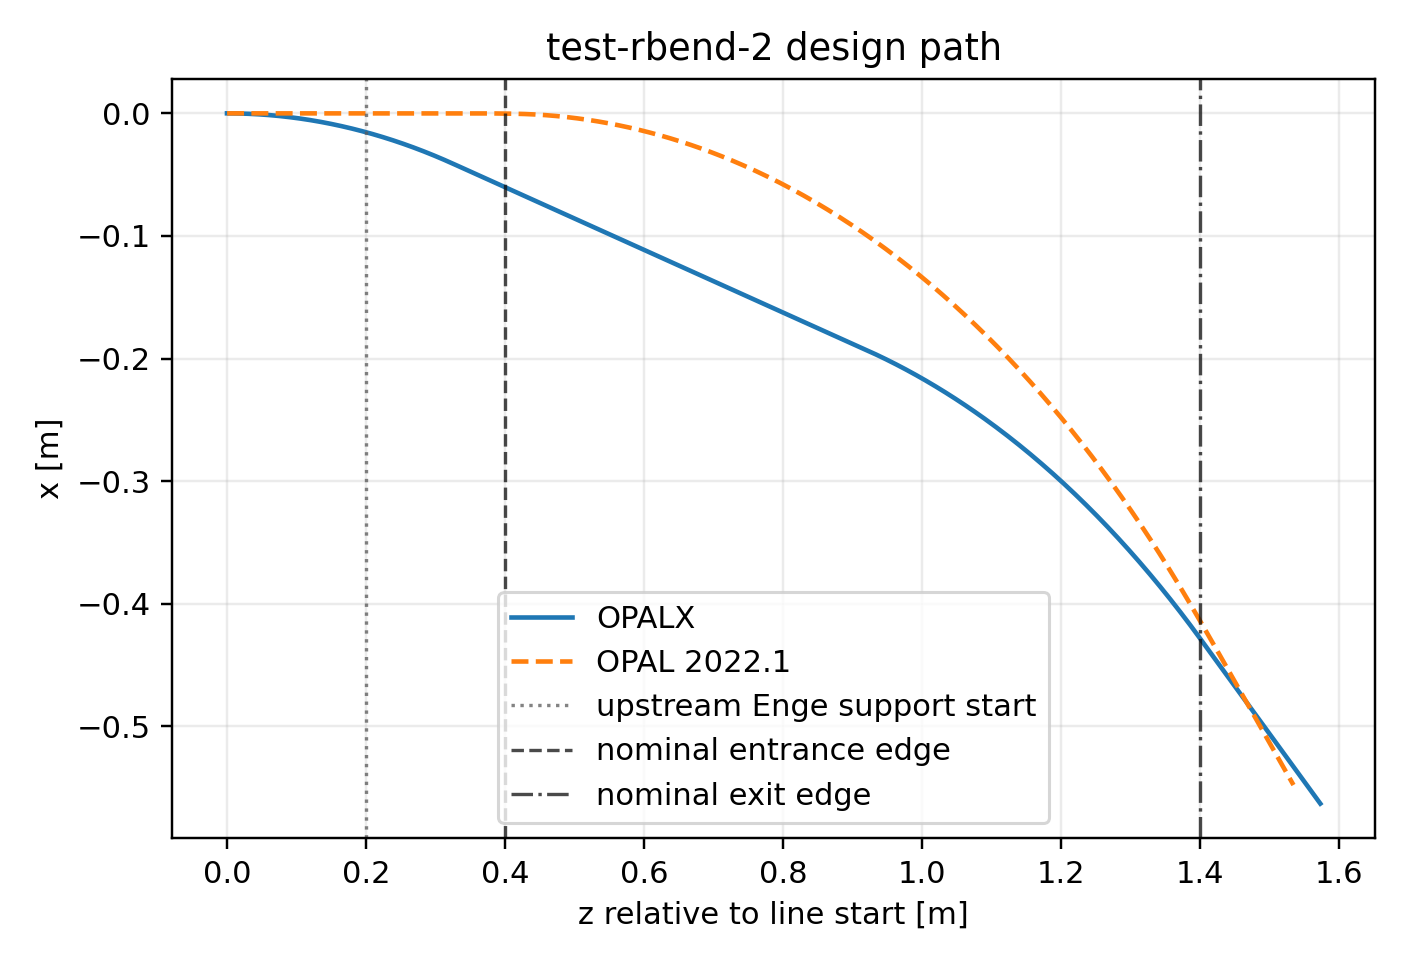
\includegraphics[width=\linewidth]{figures/test-rbend-2-design-path-xz.png}
\end{minipage}\hfill
\begin{minipage}{0.49\textwidth}
\centering
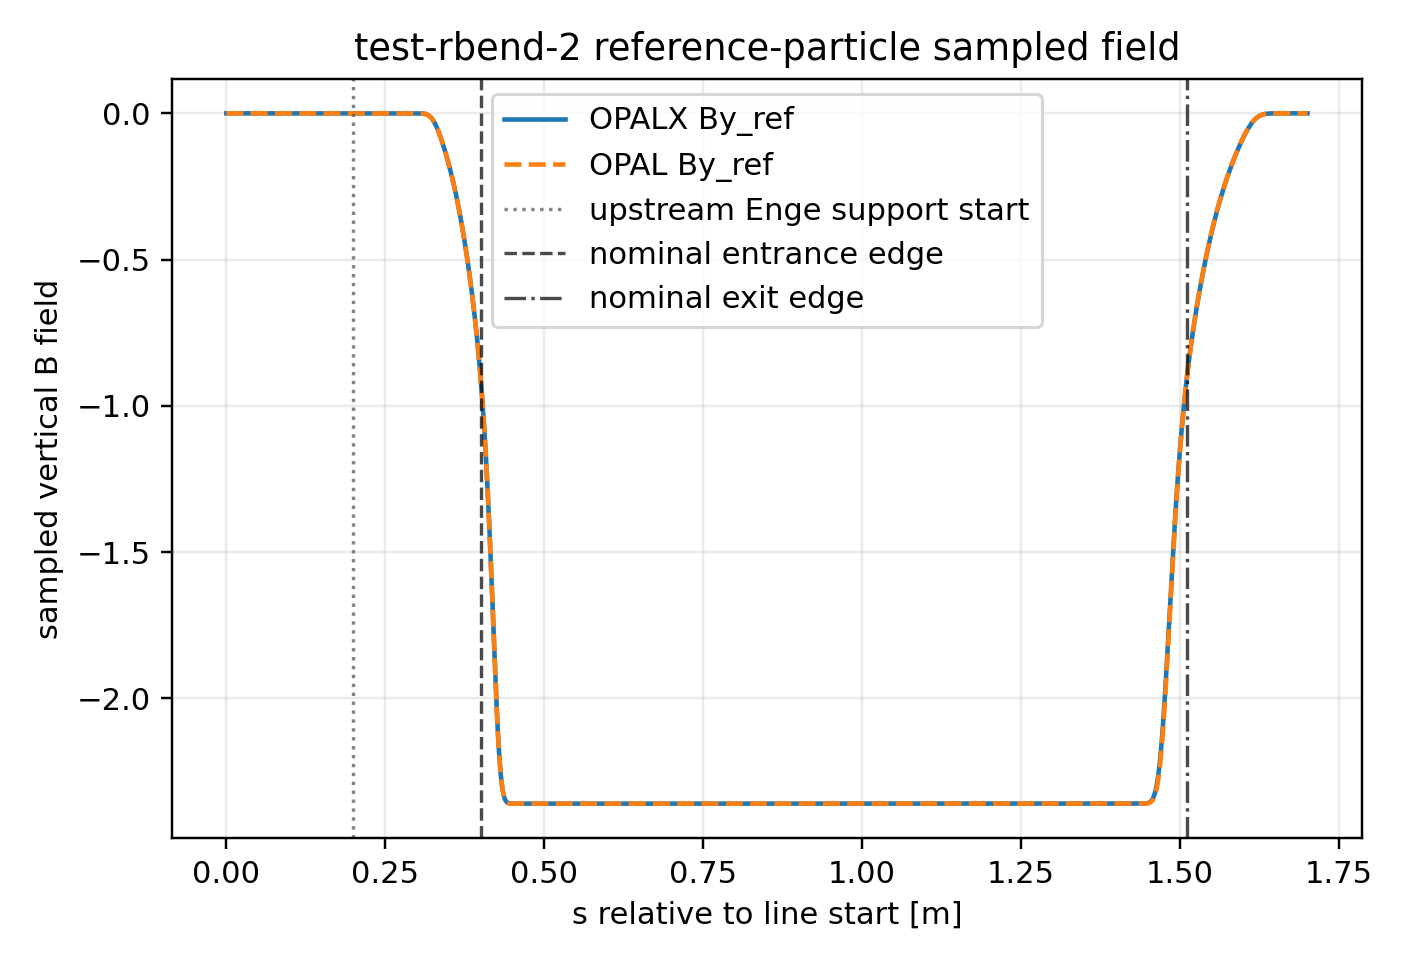
\includegraphics[width=\linewidth]{figures/test-rbend-2-stat-by-ref.png}
\end{minipage}
\caption{\code{test-rbend-2} OPALX versus OPAL 2022.1: design-path
\(X\)-\(Z\) orbit (left) and \code{.stat} reference \(B_y\) (right).}
\end{figure}

\begin{figure}[htbp]
\centering
\begin{minipage}{0.49\textwidth}
\centering
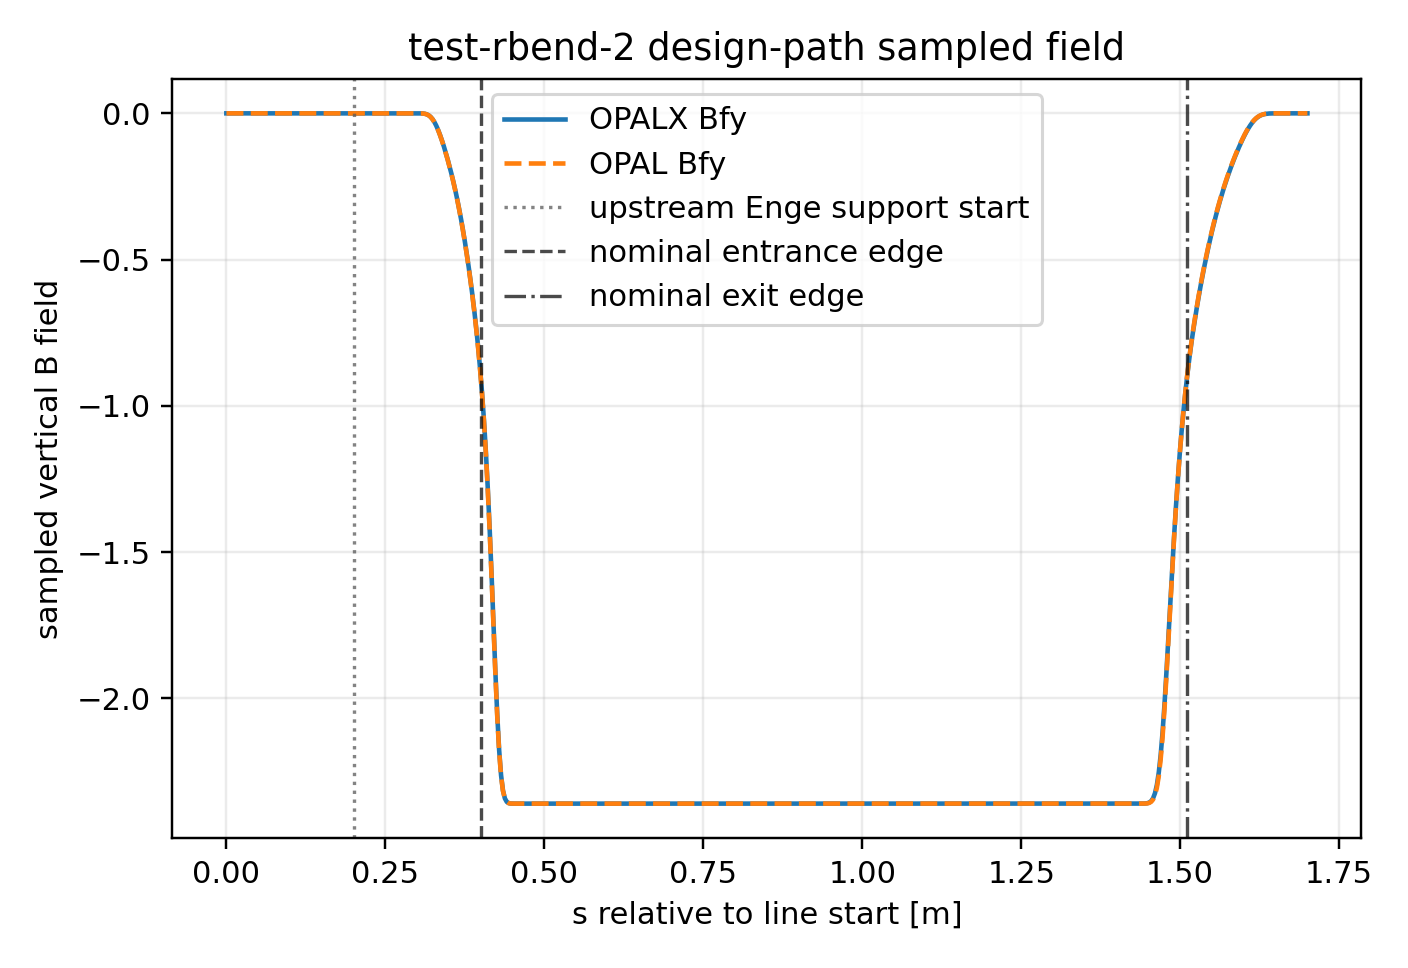
\includegraphics[width=\linewidth]{figures/test-rbend-2-design-path-by.png}
\end{minipage}\hfill
\begin{minipage}{0.49\textwidth}
\centering
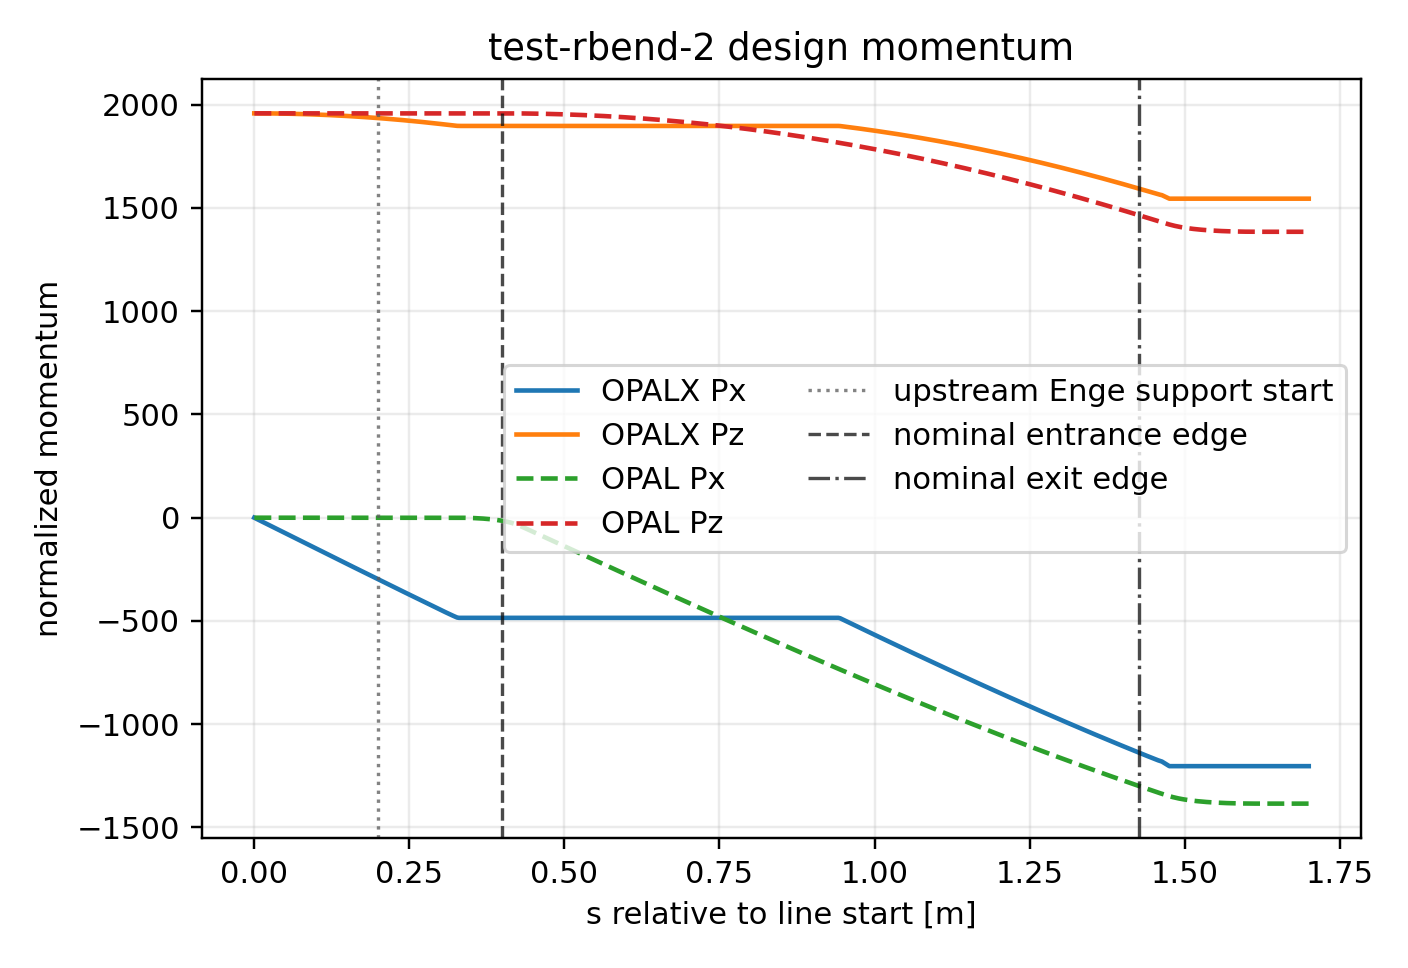
\includegraphics[width=\linewidth]{figures/test-rbend-2-design-path-momentum.png}
\end{minipage}
\caption{\code{test-rbend-2} design-path diagnostic comparison.  The marker
positions use the OPAL pole-face RBEND reference path for \(s_\mathrm{rel}\)
and the straight rectangular body length for \(z_\mathrm{rel}\).}
\end{figure}

\begin{figure}[htbp]
\centering
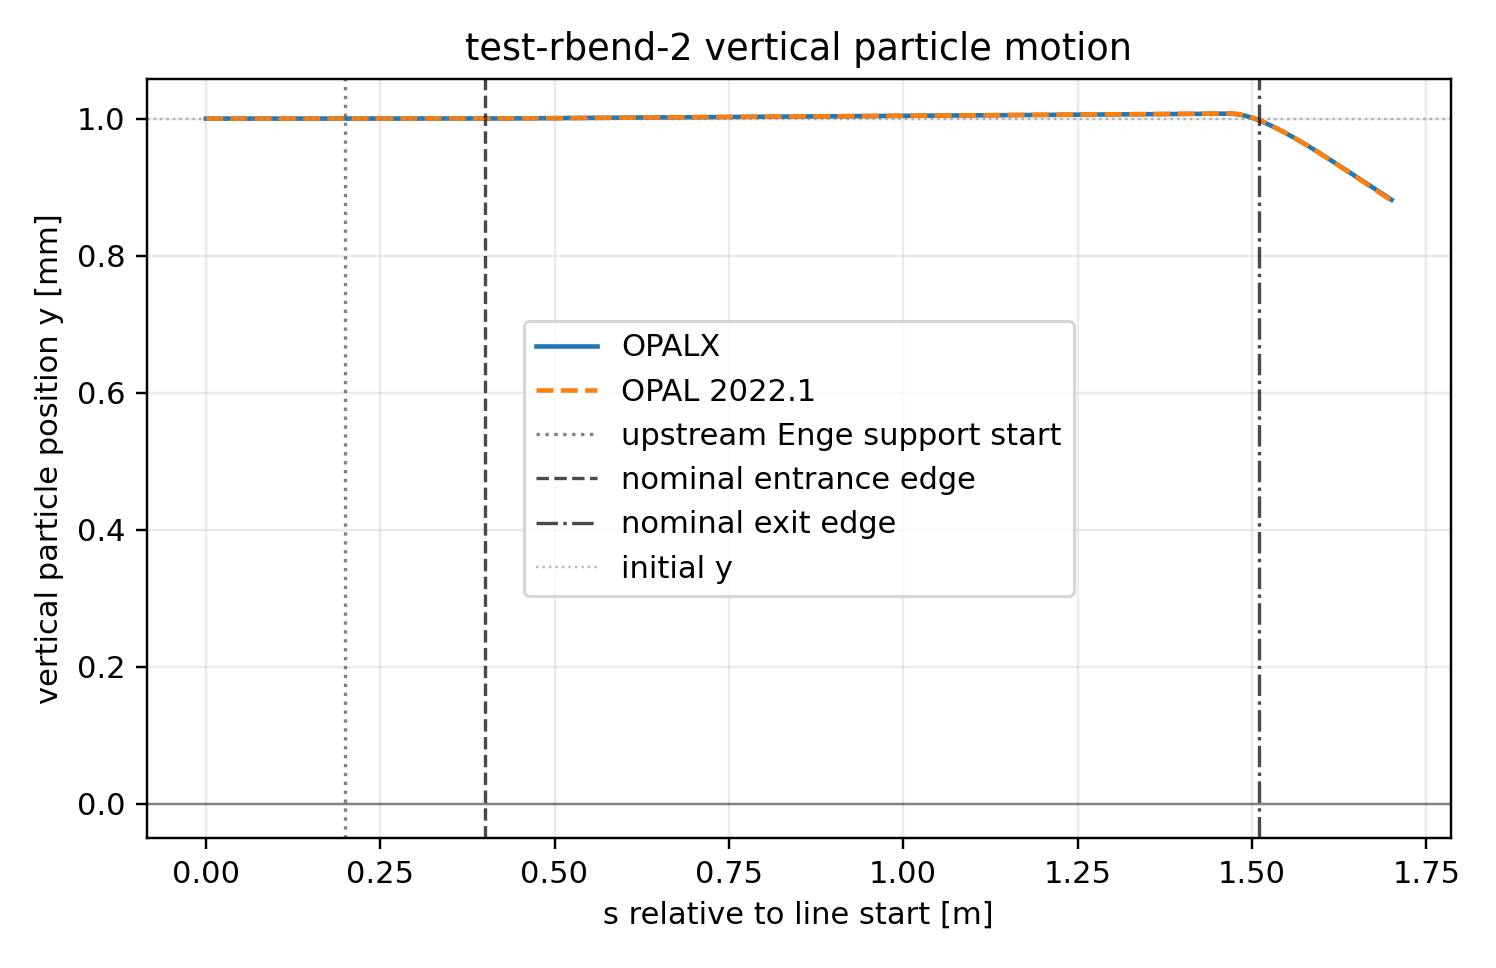
\includegraphics[width=0.78\linewidth]{figures/test-rbend-2-vertical-particle-motion.png}
\caption{\code{test-rbend-2} vertical particle motion from the \code{.stat}
\(\bar y\) column.  The final OPALX--OPAL difference is
\(1.30\times10^{-6}\ \mathrm{m}\).}
\end{figure}

\section{\code{test-chicane-1}: symmetric C-shape four-bend chicane}

Two sources are useful for a regression design.  The
USPAS bunch-compression slides give the standard four-rectangular-dipole
chicane model and the small-angle expression for \(R_{56}\)
\cite{uspas2014bunchcompression}.  The CAS FEL/ERL proceedings discuss the
symmetric C-shape chicane as a common FEL compressor geometry and give the
same small-angle model together with the usual higher-order longitudinal
coefficients \cite{dimitri2018}.

\begin{center}
\begin{tabular}{@{}lll@{}}
\toprule
source & useful content & benchmark role \\
\midrule
USPAS 2014 & four rectangular dipoles, \(R_{56}\), compression map &
primary analytic seed \\
CAS FEL/ERL & C-shape geometry, \(T_{566}\), \(U_{5666}\), timing model &
cross-check and context \\
\bottomrule
\end{tabular}
\end{center}

The OPALX benchmark is a symmetric C-shape chicane with four equal hard-edge
dipoles,
\[
  (+\theta,\,-\theta,\,-\theta,\,+\theta),
\]
magnetic length \(L_b\), lateral drift \(D\) between dipoles 1--2 and 3--4,
and central drift \(C\) between dipoles 2--3.  To leading order in
\(\theta\), the central drift does not contribute to the longitudinal
dispersion.  The school-formula target is therefore
\[
  R_{56}
    \simeq
    -\theta^2\left(\frac{4}{3}L_b + 2D\right)
    =
    -2\theta^2\left(D+\frac{2}{3}L_b\right).
\]
For the same small-angle model one can use
\[
  T_{566} \simeq -\frac{3}{2}R_{56},
  \qquad
  U_{5666} \simeq 2R_{56},
\]
as optional higher-order checks once the linear regression is promoted beyond
the present linear \(R_{56}\) probe.

The executable OPALX realization is
\[
  \code{sandbox/test-chicane-1/test-chicane-1.in}.
\]
It keeps the survey formulas symbolic in the input file.  With
\[
  \rho=\frac{L_b}{2\sin(\theta/2)},
\]
where \(L_b\) is the OPAL/OPALX \code{SBEND} chord length, not the circular arc
length, the reused survey increments are
\[
\begin{aligned}
  \Delta x_b &= \rho(1-\cos\theta),
  &\Delta z_b &= \rho\sin\theta,\\
  \Delta x_{b/2} &= \rho\left(1-\cos\frac{\theta}{2}\right),
  &\Delta z_{b/2} &= \rho\sin\frac{\theta}{2},\\
  \Delta x_{r/2} &= \rho\left(\cos\frac{\theta}{2}-\cos\theta\right),
  &\Delta z_{r/2} &= \rho\left(\sin\theta-\sin\frac{\theta}{2}\right),\\
  \Delta x_D &= D\sin\theta,
  &\Delta z_D &= D\cos\theta .
\end{aligned}
\]
The \code{REAL} symbols \code{B1\_X}, \code{B1\_Z}, \ldots,
\code{MEXIT\_X}, \code{MEXIT\_Z} in the input are assembled from these
increments and are then used directly in the element \code{X}, \code{Y},
\code{Z}, and \code{THETA} attributes.

The old OPAL comparison input is
\[
  \code{sandbox/test-chicane-1/test-chicane-1\_opal.in}.
\]
It uses old OPAL 2022.1 \code{PARALLEL-T} tracking with the same bend signs and
the same five-particle momentum scan.  In the old OPAL deck the chicane starts
at \(s=1\ \mathrm{m}\); this shifts the absolute monitor \code{SPOS}, but not
the fitted local monitor \(z\) slope used for \(R_{56}\).

\subsection{Placement result}

The OPALX run exports the requested C-chicane survey in the generated
element-position text file.  The useful placement rows are the
\code{ENTRY EDGE} and \code{EXIT EDGE} rows for the four bends:

\begin{center}
\begin{tabular}{@{}lrr@{}}
\toprule
point & \(z\) [m] & \(x\) [m] \\
\midrule
\code{B1} entry & 0.000000000 & 0.000000000 \\
\code{B1} exit / \code{D12} begin & 0.998750260 & 0.049979169 \\
\code{B2} entry & 2.491256508 & 0.199729294 \\
\code{B2} exit / \code{D23} begin & 3.490006768 & 0.249708463 \\
\code{B3} entry & 5.490006768 & 0.249708463 \\
\code{B3} exit / \code{D34} begin & 6.488757029 & 0.199729294 \\
\code{B4} entry & 7.981263276 & 0.049979169 \\
\code{B4} exit / \code{MEXIT} & 8.980013537 & 0.000000000 \\
\bottomrule
\end{tabular}
\end{center}

Compared with the symbolic survey formulas above, the largest residuals in the
exported OPALX edge table are
\[
  \max|\Delta z| = 8.28\times10^{-10}\ \mathrm{m},
  \qquad
  \max|\Delta x| = 8.33\times10^{-11}\ \mathrm{m}.
\]
The final exit monitor is therefore centered on the design exit and parallel to
the entrance axis at the precision of the exported table.

\subsection{\(R_{56}\) result}

The input carries five particles with
\[
  \delta = -2\times10^{-3},\,-10^{-3},\,0,\,+10^{-3},\,+2\times10^{-3}.
\]
The exit temporal monitor writes one local \(z\) coordinate for each particle.
The fit uses the local monitor coordinate
\[
  z_\mathrm{monitor}(\delta) - z_\mathrm{monitor}(0)
    \simeq -R_{56}\,\delta .
\]
The local monitor convention has the opposite sign from the usual transport
coefficient for this chicane, so the reported number is
\[
  R_{56} = -\frac{d z_\mathrm{monitor}}{d\delta}.
\]

\begin{center}
\resizebox{\linewidth}{!}{%
\begin{tabular}{@{}lrrrr@{}}
\toprule
case & \code{SPOS} [m] & \(d z_\mathrm{monitor}/d\delta\) [m]
     & \(R_{56}\) [m] & \(R_{56}-R_{56}^{\mathrm{target}}\) [m] \\
\midrule
small-angle target & -- & -- & \(-4.333333333333\times10^{-2}\) & -- \\
OPALX & 9.001701201 & \(+4.334628765519\times10^{-2}\)
      & \(-4.334628765519\times10^{-2}\) & \(-1.295432185213\times10^{-5}\) \\
OPAL 2022.1 & 10.003564372 & \(+4.337546378253\times10^{-2}\)
            & \(-4.337546378253\times10^{-2}\) & \(-4.213044919685\times10^{-5}\) \\
\bottomrule
\end{tabular}
}
\end{center}

The OPALX result differs from the old OPAL result by
\[
  R_{56,\mathrm{OPALX}} - R_{56,\mathrm{OPAL}}
    = 2.92\times10^{-5}\ \mathrm{m}.
\]
Both codes are close to the small-angle school formula; the remaining
difference is expected at this level because the comparison uses finite
\(\theta=0.1\ \mathrm{rad}\), finite integration steps, and a monitor-based
local-coordinate extraction rather than a strict first-order transfer map.

\begin{figure}[htbp]
\centering
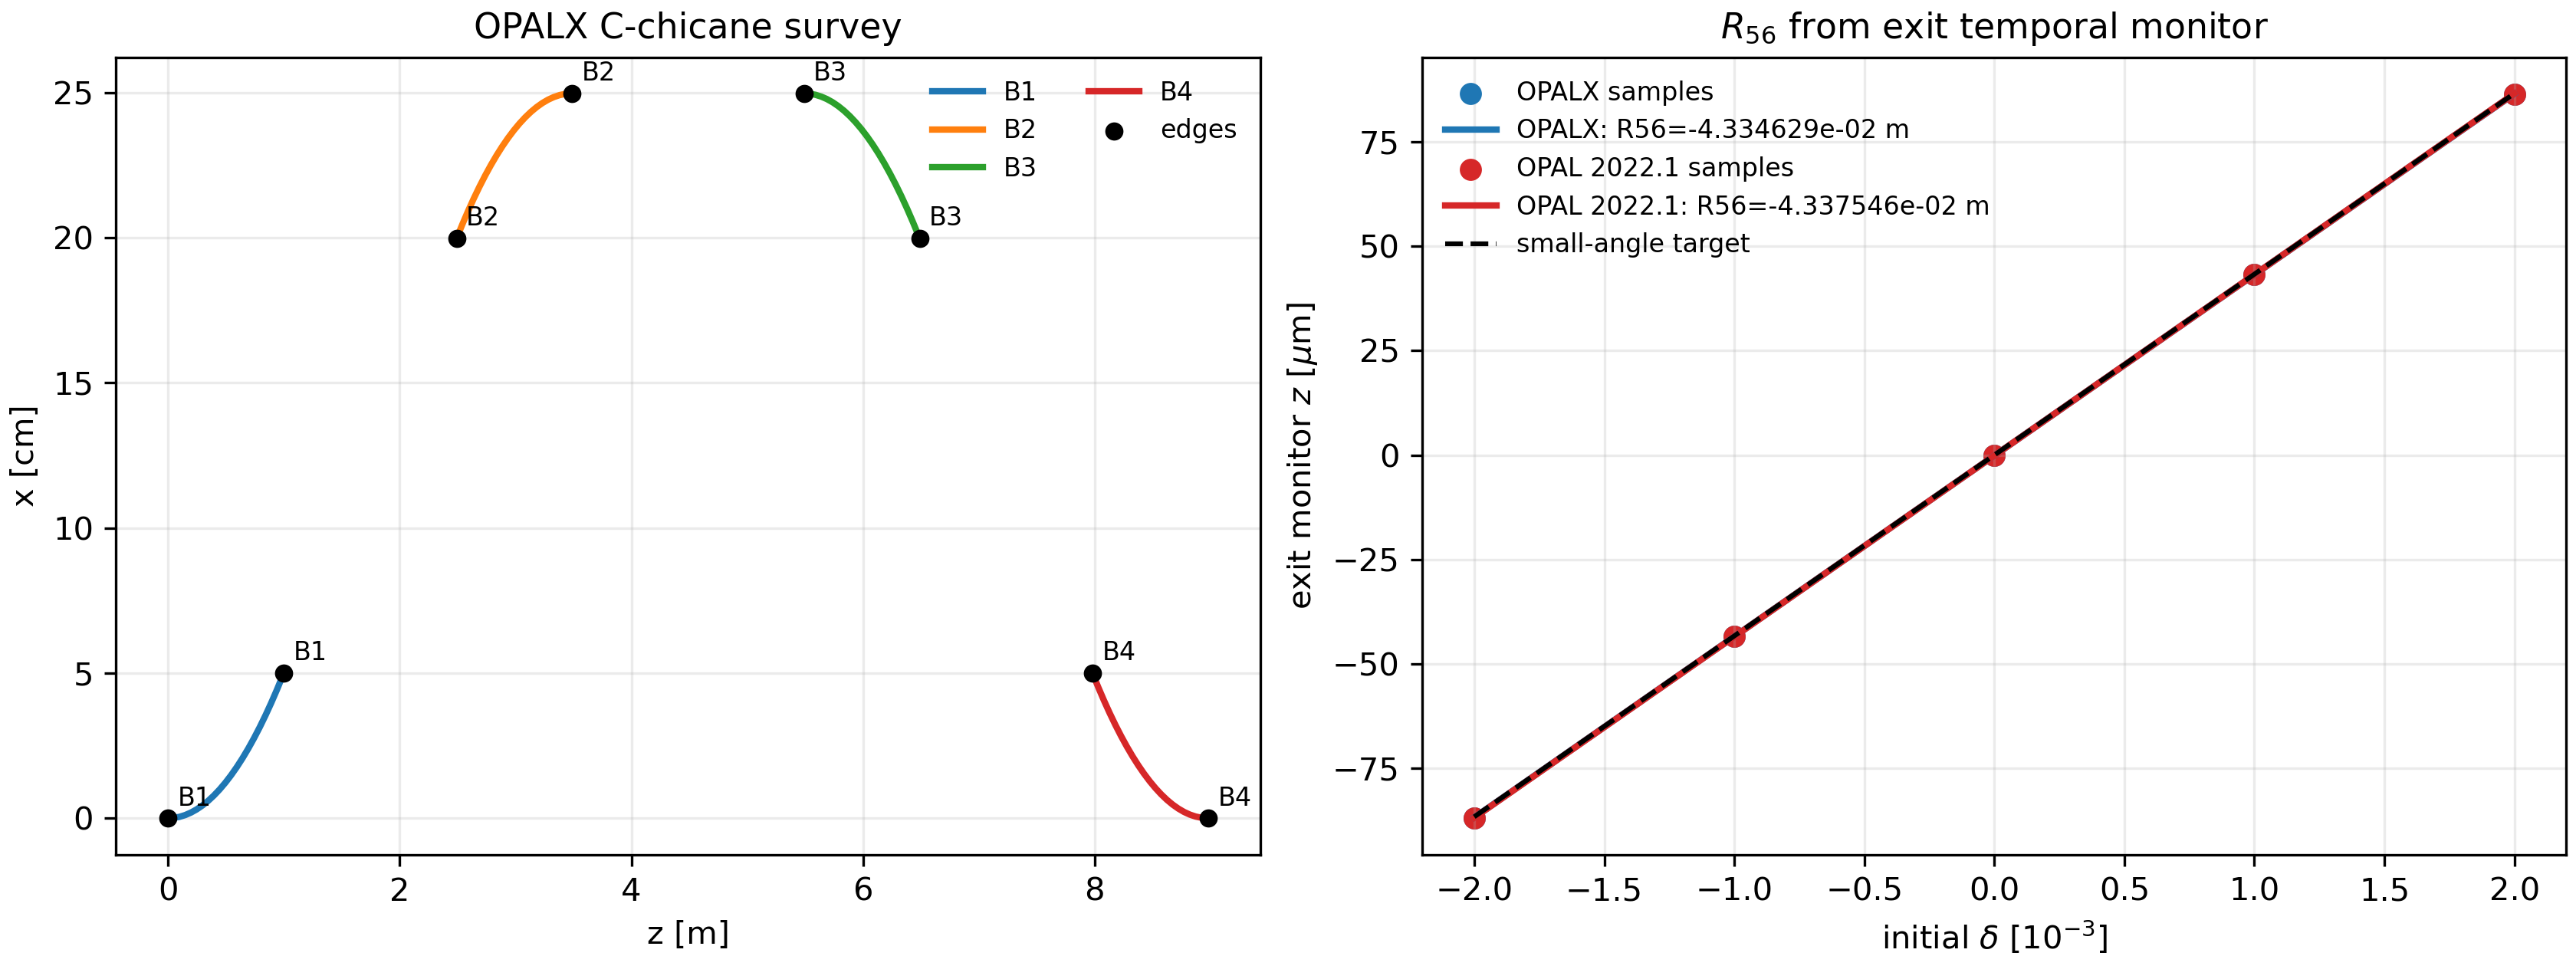
\includegraphics[width=\linewidth]{figures/test-chicane-1-survey-r56.png}
\caption{\code{test-chicane-1} results.  Left: OPALX exported C-chicane survey
from the bend edge and midpoint rows.  Right: exit temporal-monitor \(z\)
versus initial \(\delta\) for OPALX and OPAL 2022.1.  The dashed line is the
small-angle \(R_{56}\) target with the monitor-sign convention applied.}
\end{figure}

\begin{thebibliography}{9}

\bibitem{holzer2018}
B.~J. Holzer,
\emph{Transverse Beam Dynamics},
CERN Yellow Reports: School Proceedings, Vol.~5 (2018),
\url{https://doi.org/10.23730/CYRSP-2018-005.1}.

\bibitem{brown1982}
K.~L. Brown,
\emph{A First- and Second-Order Matrix Theory for the Design of Beam Transport
Systems and Charged Particle Spectrometers},
SLAC-R-075, Rev.~4, June 1982,
\url{https://www.slac.stanford.edu/pubs/slacreports/reports01/slac-r-075.pdf}.

\bibitem{madx}
H.~Grote, F.~Schmidt, L.~Deniau, and G.~Roy,
\emph{The MAD-X Program: User's Reference Manual},
CERN, Version 5.02 series, sections on reference-system poses, \code{SBEND}, and
dipole-edge focusing,
\url{https://madx.web.cern.ch/}.

\bibitem{bmad}
D.~Sagan,
\emph{Bmad Manual},
Cornell CLASSE, sections on \code{SBEND}/\code{RBEND}, bend coordinates, and
fringe-field integrals,
\url{https://www.classe.cornell.edu/bmad/bmad-manual.pdf}.

\bibitem{elegant}
M.~Borland,
\emph{elegant: A Flexible SDDS-Compliant Code for Accelerator Simulation},
Advanced Photon Source, sections on \code{CSBEND} and \code{RBEN},
\url{https://ops.aps.anl.gov/manuals/elegant_latest/elegant.html}.

\bibitem{uspas2014bunchcompression}
D.~Nguyen, J.~Lewellen, and L.~Duffy,
\emph{RF Linac for High-Gain FEL: Bunch Compression},
US Particle Accelerator School, June 2014,
\url{https://uspas.fnal.gov/materials/14UNM/E_Bunch_Compression.pdf}.

\bibitem{dimitri2018}
S.~Di Mitri,
\emph{Bunch-Length Compressors},
Proceedings of the CAS-CERN Accelerator School on Free Electron Lasers and
Energy Recovery Linacs, CERN Yellow Reports: School Proceedings, Vol.~1 (2018),
\url{https://doi.org/10.23730/CYRSP-2018-001.361}.

\end{thebibliography}

\end{document}
